\documentclass[11pt]{article}
%\documentclass[11pt,twocolumn,letterpaper]{article}
\setlength{\columnwidth}{8.6cm}
\setlength{\textheight}{23cm}
\setlength{\topmargin}{-0.8cm}
%\documentclass[11pt]{article}
\usepackage{graphicx}
\usepackage{verbatim}
\usepackage{color}
\usepackage{url}
\usepackage{longtable}
\usepackage{hyperref}
%\usepackage{booktabs}
%\usepackage{amssymb,amsmath}
%\usepackage[dvips]{color, graphics, epsfig, graphicx}
\bibliographystyle{unsrt}
%\bibliographystyle{apsrev.bst}
%\topmargin 0mm 
%\textheight 220mm
%\textwidth 160mm
%\oddsidemargin 5mm
%\mathsurround 2pt

%\renewcommand{\textfraction}{0.10}
%\renewcommand{\topfraction}{0.85}
%\renewcommand{\bottomfraction}{0.65}
%\renewcommand{\floatpagefraction}{0.60}
%\renewcommand{\thetable}{\Roman{table}}

%\setcounter{figure}{7}
%\setcounter{table}{8}

\begin{document}

\author{
  Andrew Jewett, \\
  Jensen Lab (Caltech), Shea Lab (UCSB) \\

\includegraphics[height=0.3cm]{author_email.png}
}
\date \today


\title{Emoltemplate Manual}



\maketitle

  \textit{\textbf{Emoltemplate is based on Moltemplate, a molecule-building tool for LAMMPS.  Similarly, this manual is based on the manual for moltemplate.  As such, there may be mistakes.  Please report inaccuracies to the author (via email or git).}}

\tableofcontents

  %Additionally, several working examples of molecules created 
  %with emoltemplate can be found in the ``examples/'' subdirectory 
  %(which is distributed with emoltemplate).
  %These were created to supplement the emoltemplate documentation.

\section{Introduction}

 Emoltemplate is a cross-platform text-based molecule builder for ESPResSo. It is typically used for building coarse-grained toy molecular models. Emoltemplate users have access to (nearly) all of the standard and non-standard (custom, user-created) force-field and features available in ESPResSo.

  %\textit{(Although optimized for ESPResSo, emoltemplate comes with a general text manipulation tool (ttree.py) which, in principle, could be used to generate topology and force-field files for other simulation programs.  Please email 
\includegraphics[height=0.3cm]{author_email.png} if you wish to attempt this.)}

A file format has been created to store molecule definitions (the ESPResSo-template format, ``ET''). Typical ``.ET'' files contain atom coordinates, topology data (bonds), ESPResSo force-field data, and other ESPResSo settings (such as user-defined input files) for a type of molecule (or a molecular subunit).  Molecules can be copied, combined, and linked together to define new molecules. (These can be used to define larger molecules. Unlimited levels of object composition, nesting, and inheritance are supported.) Once built, individual molecules and subunits can be customized (atoms and bonds, and subunits can be moved, deleted and replaced).

  %Existing ESPResSo input/data files can be converted into ``ET'' format using the ``etemplify.py'' utility.

Emoltemplate requires the Bourne-shell, and a recent version of python (2.7 or 3.0 or higher), and can run on OS X, linux, or windows (if a suitable shell environment has been installed).  Memory requirements are discussed in {sec:limitations}.

  %Emoltemplate is a text-manipulation tool for generating 
  %input files for molecular dynamics simulation programs.
  %Emoltemplate has been optimized for constructing input files for ESPResSo.
     %from constituent parts.
  %Molecules are stored in a hierarchical, 
  %object-oriented, 
  %template-based file format (``.ET'').
  %   %using an object-oriented style 
  %   %which can mimic many popular molecular file formats.
  %  %such as PDB, amber TOP, Gromacs TOP, 
  %  %PSF files, and some limited xplor parameter files.
  %  %existing ESPResSo file formats. 
  %Typical ``.ET'' files contains ESPResSo force-field data, 
  %topology data, and other settings (such as auxiliary files)
  %for any molecule or repeating subunit. 
  %These subunits can be combined together 
  %to build larger, more complicated systems.
  %With unlimited levels of nesting, object composition, and inheritance, 
  %these objects can be combined to build
  %elaborate heterogeneous molecular assemblies.


%  %%Emoltemplate can also be used to automatically detect 
%  %%topological relationships between bonded atoms and determine 
%  %%(the parameters of) the forces between them accordingly.
%  %Emoltemplate also extends basic ESPResSo functionality.
%  %It can also be used to automatically detect 
%  %bonded many-body interactions (such as dihedrals), 
%  %and programmed to determine (the parameters of) 
%  %the forces between them according to atom and bond type.
%  %This makes the ET-file format useful in general 
%  %for storing force-field parameters.
%
%ET files can also be used for storing force-fields 
%for molecules whose topology has not yet been determined. 
%Emoltemplate automatically detects 
%  % topological relationships between bonded atoms and 
%bonded many-body interactions (such as dihedrals), 
%and can determine (the parameters of) 
%the forces between them according to atom and bond type. 
%Once a system's geometry and bonds have been specified, 
%a user can apply completely different force fields to the existing system 
%by loading a different ET file containing force-field parameters. 
%

\subsection{Converting \textit{ET files} to ESPResSo TCL commands}
The emoltemplate.sh program converts ET-files (which contain 
molecule definitions) into a file containing ESPResSo TCL commands:
\begin{verbatim}
emoltemplate.sh system.et
\end{verbatim}
     or
\begin{verbatim}
emoltemplate.sh -xyz coords.xyz system.et
\end{verbatim}
In the first example, the coordinates of the atoms in the 
system are built from commands inside the ``system.et'' file.
In the second example coordinates for the atoms are 
read from an XYZ-file (PDB-files are also supported).
(The ``full'' atom style was used in this example, but other
 ESPResSo atom styles are supported, including hybrid styles.)

Either of these commands will construct a ESPResSo TCL file 
(and possibly one or more auxiliary input files),
which can be directly run in ESPResSo with minimal editing.


  %\subsection{Converting ESPResSo input/data files to \textit{ET files}}
  %Existing ESPResSo input/data files can be converted into 
  %  %espresso-template 
  %``.ET'' files using the ``etemplify.py'' utility.
  %(See appendix \ref{sec:etemplify}.)

%\subsection*{Strengths}
%Emoltemplate is especially useful for defining new, exotic 
%coarse-grained molecular models natively from scratch.
%Molecules defined this way have access to (nearly)
%\textit{all} of the 
%  %extraordinary 
%  bewildering 
%menu of features and force-fields
%available in ESPResSo.  This includes custom ESPResSo features 
%created by end-users (now and probably in the future).
%
%   %The ``.ET'' file format is \textit{not} specific to ESPResSo and 
%   %can also be useful for generating other files which store molecular data.
%  %ET files are text templates.
%ET files are very flexible and can mimic almost any text file format 
%which uses simple numerical counters.
%End users can accommodate gradual changes in the ESPResSo input and data file 
%formats by altering their own molecule templates 
%as ESPResSo independently grows and evolves.

%\subsection*{Limitations}
%  %Little effort has yet been made to allow emoltemplate.sh to read and write
%  %simulation files from other programs.
%Emoltemplate.sh was \textit{not} designed to work seamlessly with 
%files from other simulation or visualization programs
%(although such functionality could be added). 
%Emoltemplate.sh does not provide a quick or convenient way to perform an 
%all-atom simulation of proteins or nucleic-acids in an box of water 
%(for example). 
%Emoltemplate has only limited support for generating molecular geometry
%and it does not have a graphical interface. 
%For these tasks, external utilities are very helpful.

\subsection*{Additional tools}
  %The VMD topotools plugin \cite{topotools} is useful for 
  %converting PDB files into ESPResSo format.  These files can then
  %be converted to ``ET'' format using the ``etemplify.py'' utility.
  %VMD and topotools are also useful for visualizing the data files 
  %created by emoltemplate.sh.
  %(Documentation for doing this is included 
  % in the \textit{online examples} discussed below.)

  %Pizza.py \cite{pizzapy}, has a utility for building 1-bead polymer melts.

  The PACKMOL \cite{packmol} program is useful for generating 
coordinates of dense heterogeneous mixtures of molecules,
which can be read by emoltemplate.
(The VMD ``solvate'' plugin may also be helpful.)
  %There are many other utilities, 
    %graphical modeling programs, 
    %and numerous scripts (which are in various stages of maintenance) 
  %which may be useful for file format conversion, and
  %pre-and-post processing and analysis.
  %Many other tools exist (not covered here) which can convert file formats 
  %used by other molecular dynamics software programs into ESPResSo format.

  VMD \cite{VMD} is very useful for visualization. 
VMD can interactively visualize ESPResSo simulations while 
they are in progress \cite{VMDIMD}.
VMD also has a number of plugins for generating molecular geometry.


\subsection*{Online examples}

  %When using ``emoltemplate.sh'' it does not hurt to have 
  %a modest familiarity ESPResSo and it's file formats,
  %because this mirrors the ``.ET'' file format described here.

This manual explains how to use emoltemplate.sh to build ESPResSo 
files from scratch, but it does not discuss how to run ESPResSo
or how to visualize the results.
%provides only a very brief overview 
%of how to run simple simulations in ESPResSo
%(see sections \ref{sec:spce_example} and \ref{sec:run}),
%and it does not discuss how to visualize or analyze ESPResSo
%simulation trajectories.

This manual assumes users have some basic familiarity with ESPResSo.

For users who are not familiar with ESPResSo, several complete, 
working examples (with images and readme files) are available online 
  (at \url{http://moltemplate.org/espresso})
which can be downloaded and modified.
  %These examples are included with the main emoltemplate download.
%(See download instructions below.)
%(which can be downloaded from the official emoltemplate web site 
%at \url{http://www.moltemplate.org/espresso}). 
%They are more complex than the examples 
%explained here in this manual. 
%The official ESPResSo examples and user manual
%are also a valuable reference.
These examples are a good starting point for learning ESPResSo and emoltemplate.



\subsection*{License}
Emoltemplate.sh is publicly available at \url{http://moltemplate.org/espresso} 
under the terms of the open-source 3-clause BSD license.
\url{http://www.opensource.org/licenses/BSD-3-Clause}







%  \subsubsection*{Using ``ettree.py'' instead of ``emoltemplate.sh''}
%  The format of an ``.ET'' file closely mimics the syntax in 
%  current ESPResSo data and input script files (as of early 2012).
%  However ESPResSo file formats are constantly changing
%  as users add their own custom features to ESPResSo. 
%  (In addition, there are some currently known limitations of 
%  emoltemplate.sh, which are discussed in section \ref{sec:limitations}.)
%    %However this file format must be flexible enough 
%    %to handle potentially radical syntax changes in the future.
%    %End users who add new features to ESPResSo may also modify the syntax 
%    %of these input files, and will likely introduce new file formats.
%  Consequently, we also provide several simple python scripts: 
%    %(which should remain useful when/if emoltemplate.sh breaks)
%  ``ttree.py'', ``ettree.py'', and ``nbody\_by\_type.py''. 
%    %\begin{list}
%    %\item 
%    %``ttree.py'', is a general text manipulation 
%    %tool which prints out the text contained in the 
%    %``write()'' and ``write\_once()'', commands in an ET file, 
%    %and substitutes numerical values into the \$ and \@ variables
%    %contained inside.
%    %\item 
%    %``ettree.py'' is a variant of ``ttree.py''
%    %  %understand ESPResSo atom\_style syntax and 
%    %which also generates atomic coordinates.
%    %(It process the ``.move()'' and ``.rot()'' commands.)
%    %\item 
%    %``nbody\_by\_type.py'' is a utility which generates 
%    %many-body bonded interactions between atoms automatically, 
%    %according to the atom and bond type.
%    %(It processes the ``Angles By Type'', 
%    %``Dihedrals By Type'', and ``Impropers By Type'' sections.)
%    %\end{list}
%  The ``ttree.py'' program is a general text manipulation tool which 
%  should continue to work in the distant future, 
%  even if the ESPResSo syntax changes radically, and ``emoltemplate.sh'' breaks. 
%  (``ttree.py'' is nearly identical to and supports all the 
%  command line options used by ``emoltemplate.sh'', 
%  with the exception of ``-pdb'' and ``-xyz''.)
%    %However this tool is intentionally simple and ignorant about ESPResSo. 
%    %This allows programmers to add features to ESPResSo without ever
%    %breaking the ``.ET'' file format.
%      %(although you may have to sacrifice some convenience
%      %that using emoltemplate.sh provides).
%  A tutorial for using these programs
%  is provided in appendix \ref{sec:ttree}.




\section{Installation}

\subsection*{Obtaining Emoltemplate}

The source code for emoltemplate is now included with \textit{moltemplate}.
To install emoltemplate, you must install moltemplate.
However the examples and documentation
which come with moltemplate are specific to LAMMPS, not ESPResSo.
%\subsubsection*{ESPResSo Documentation}
ESPResSo-specific documentation and examples are now a separate download.
Links to \textit{both} the documentation/examples, \textit{as well as} the
moltemplate source code can be found at:
\url{http://www.moltemplate.org/espresso/download.html}
%\subsubsection*{tar.gz Archives}
If you obtained moltemplate or emoltemplate as a .tar.gz file,
(as opposed to github), then you can unpack it using:
\begin{verbatim}
tar -xzvf emoltemplate_2016-12-08.tar.gz
\end{verbatim}
(The date will vary from version to version.)
Sometimes this archive includes the moltemplate source code.
In that case, the directory will contain a subdirectory named ``moltemplate''
containing the moltemplate source code and python packaging files.

If necessary, move the (outermost) \textit{``moltemplate''} directory to its 
desired location. (For the sake of this example, let's assume it is located
in your home directory.
\textit{\textbf{Note:} This directory should contain the file
        ``\textbf{setup.py}''})

There are two ways to install moltemplate/emoltemplate:

\subsubsection*{Installation Method 1 (pip)}

\textit{If you are familiar with pip}, then run this command from within
the \textit{moltemplate} directory:
\begin{verbatim}
pip install .
\end{verbatim}

%\textit{In order for this to work, this directory should contain a file named ``\textbf{setup.py}''.}  (If no such file exists, then either proceed to ``Installation Method 2'' below, or download a newer version of emoltemplate.)

Make sure that your default pip install bin directory is in your PATH.  (This is usually something like ~/.local/bin/ or ~/anaconda3/bin/.  If you have installed anaconda, your PATH should have been updated for you automatically.)  Later, you can uninstall both moltemplate/emoltemplate using:
\begin{verbatim}
pip uninstall moltemplate
\end{verbatim}
Instructions for updating your PATH are included below.


\subsubsection*{Installation Method 2}

Alternatively, you can edit your PATH variable manually to include
the subdirectory where the emoltemplate.sh script is located 
(typically ``moltemplate/moltemplate/scripts/''), as well as 
the directory containing the most of the python scripts (``moltemplate/'').
Suppose the project directory with the README file is named
``emoltemplate'', and suppose it is located in your home directory:

If you use the \textbf{bash} shell, typically you would edit your 
\mbox{$\sim$/.bash\_profile}, 
\mbox{$\sim$/.bashrc}, or 
\mbox{$\sim$/.profile} files
and append the following lines:
\begin{verbatim}
export PATH="$PATH:$HOME/moltemplate/moltemplate"
export PATH="$PATH:$HOME/moltemplate/moltemplate/scripts"
\end{verbatim}
If instead you use the \textbf{tcsh} shell, typically you would edit your 
\mbox{$\sim$/.login}, 
\mbox{$\sim$/.cshrc}, or 
\mbox{$\sim$/.tcshrc} files 
and append the following lines:
\begin{verbatim}
seetnv PATH "$PATH:$HOME/moltemplate/moltemplate"
setenv PATH "$PATH:$HOME/moltemplate/moltemplate/scripts"
\end{verbatim}


\textit{Note: You may need to log out and then 
log back in again for the changes to take effect.}



\pagebreak
\section{Quick reference \textit{(skip on first reading)}}

\section*{
\textit{Note: New users should skip to section \ref{sec:tutorial}}
}



\subsection{Emoltemplate commands}

%\begin{table}
\begin{longtable}[h]{l|p{9cm}}
\textbf{command} & \textbf{meaning}
\\
\hline
\hline
\begin{tabular}[t]{l}
\\
\textit{MolType} \textbf{\{} \\
\\
\hspace{0.35cm} \textit{content} ... \\
\\
\textbf{\}} \\
\end{tabular}
& 
Define a new type of molecule (or namespace) named \textit{MolType}.
The text enclosed in curly brackets (\textit{content})
typically contains multiple write(), write\_once()
commands to define Atoms, Bonds, Angles, Coeffs, etc...
\textit{(If that molecule type exists already, 
then this will append additional \textbf{content} to its definition.)}
\textbf{new} and \textbf{delete} commands can be used 
to create or delete molecular subunits \textit{within} this molecule.
(See the \textit{SPCEflex}, \textit{Monomer}, and \textit{Butane} 
 molecules, and the \textit{TraPPE} namespace 
 defined in sections \ref{sec:spce_example}, \ref{sec:2bead},
 \ref{sec:inheritance}, \& \ref{sec:trappe}.
\\
\hline
\textit{mol\_name} = \textbf{new} \textit{MolType} &
Create (instantiate) a copy of a molecule of type \textit{MolType}
and name it \textit{mol\_name}.
(See section \ref{sec:spce_example}.)
\\
\hline
\textit{mol\_name} = \textbf{new} \textit{MolType}.\textit{xform()} &
Create a copy of a molecule and
apply coordinate transformation \textit{xform()} to its coordinates.
(See sections \ref{sec:coords_intro} and \ref{sec:xforms_table}.)
\\
\hline
\textit{molecules} = 
  \textbf{new} \textit{MolType} [\textit{N}].\textit{xform()}&
Create \textit{N} copies of a molecule of type \textit{MolType}
and name them 
\textit{molecules[0]}, \textit{molecules[1]}, \textit{molecules[2]}...
Coordinates in each successive copy are cumulatively transformed 
according to \textit{xform()}.
(See sections \ref{sec:coords_intro}, \ref{sec:arrays+xform}
and \ref{sec:xforms_table}.)
Multidimensional arrays are also allowed.
(See section \ref{sec:multidimensional_arrays}.)
\\
\hline
\begin{tabular}[t]{l}
\textit{molecules} = \textbf{new} \textit{MolType.xform1()}
\\
\hspace{3.7cm}            \textbf{[\textit{N}]}.\textit{xform2()}
\\
\end{tabular}
&
Apply coordinate transformations (\mbox{\textit{xform1()}}
to \mbox{\textit{MolType}}, before making \textit{N} copies
of it while cumulatively applying \mbox{\textit{xform2()}}.
(See section \ref{sec:xform+arrays+xform} and \ref{sec:xform_order}.)
\\
\hline
\begin{tabular}[t]{l}
\textit{molecules} = \textbf{new} 
\\
    \hspace{0.6cm} \textbf{random}([\textit{M1.xf1()}, 
\\
    \hspace{2.3cm}                  \textit{M2.xf2()},
\\
    \hspace{2.3cm}                  \textit{M3.xf2()},...],
\\
    \hspace{2.25cm}        [$p_1$, $p_2$, $p_3$,...],
\\
    \hspace{2.25cm}         \textit{seed})
\\
    \hspace{0.6cm}    \textbf{[\textit{N}]}.\textit{xform()}
\end{tabular}
&
Generate an array of \textit{N} molecules randomly selected from 
\mbox{\textit{M1,M2,M3,...}}
with probabilities \mbox{$p_1, p_2, p_3$...},
using (optional) initial coordinate transformations
\textit{xf1(), xf2(), xf3, ...}, and applying transformation \textit{xform()}
cumulatively thereafter.
This also works with multidimensional arrays.
(See sections \ref{sec:random_arrays} and \ref{sec:random_advanced}.)
\\
\hline
\textit{NewMol} = \textit{OldMol} &
Create a new molecule \textbf{type} based on an existing molecule type.
Additional atoms (or bonds, etc...) can be added later to the new molecule 
using \mbox{NewMol \{\textit{more\ content}...\}}.  
(See section \ref{sec:molecule_customization}.)
\\
\hline
\textit{NewMol} = \textit{OldMol}.\textit{xform()}
&
Create a new molecule \textbf{type} based on an existing molecule type,
and apply coordinate transformation \textit{xform()} to it.
(See section \ref{sec:molecule_customization}.)
\\
\hline
  %\textit{NewMol} \textbf{inherits} \textit{Mol1} \textit{Mol2} \mbox{\{...\}} &
\begin{tabular}[t]{l}
\textit{NewMol} \textbf{inherits} \textit{Mol1} \textit{Mol2} ... \{ \\
\\
\hspace{0.35cm} \textit{additional content} ... \\
\\
\} \\
\end{tabular}
&
Create a new molecule \textbf{type} based on multiple existing molecule types.
Atom types, bond types, angle types (etc) which are defined in
\textit{Mol1}, or \textit{Mol2}, ... are available inside the
new molecule.
\textit{Additional content} 
(including more \textit{write()} or \textit{write\_once()}
or \textit{new} commands)
follows within the curly brackets.
(See sections \ref{sec:inheritance_intro},
\ref{sec:inheritance}, and \ref{sec:multiple_inheritance})
\\
\hline
\textit{MolType}.\textit{xform()}
&
Apply the coordinate transform \textit{xform()} to the coordinates 
of the atoms in all molecules of type \textit{MolType}.
(See section \ref{sec:molecule_customization}.
\\
\hline
\textit{molecule}.\textit{xform()}
&
Apply the coordinate transform \textit{xform()} 
to the coordinates in \textit{molecule}.
(Here \textit{molecule} refers to a specific instance or copy of
 a particular molecule type.
See sections \ref{sec:custom_xform} and \ref{sec:coords_intro}.)
\\
\hline
\textit{molecules}[\textit{range}].\textit{xform()}
&
Apply the coordinate transform \textit{xform()} 
to the coordinates of molecules specified by
\mbox{\textit{molecule}[\textit{range}]}.
(This also works for multidimensional arrays.
See sections \ref{sec:array_wildcards_intro} and \ref{sec:custom_xform}.)
\\
\hline
\textbf{delete} \textit{molecule}
&
Delete the \textit{molecule} instance.
(This command can appear inside a molecule's definition 
 to delete a specific molecular subunit within a molecule.  In that case,
 it will be carried out in every copy of that molecule type.
 \textbf{delete} can also be used to delete specific
 atoms, bonds, angles, dihedrals, and improper interactions.)
See section \ref{sec:delete}.
\\
\hline
\textbf{delete} \textit{molecules}[\textit{range}]
&
Delete a range of molecules specified by 
\mbox{\textit{molecule}[\textit{range}]}.
(This also works for multidimensional arrays.
 See sections \ref{sec:delete} and \ref{sec:delete_holes}.)
\\
\hline
  %\mbox{write\_once}('\textit{file}') \mbox{$\{$\textit{text}\ldots$\}$} & 
\begin{tabular}[t]{l}
\textbf{write\_once}('\textit{file}') \{ \\
\hspace{0.35cm} \textit{text} ... \\
\} \\
\end{tabular} &
Write the text enclosed in curly brackets \mbox{$\{\ldots\}$}
to file \mbox{$file$}. 
The \textit{text} can contain @variables which are replaced by integers.
(See sections \ref{sec:write} and \ref{sec:variables}.)
\\
\hline
  %\textit{write}('file') \mbox{$\{text\ldots{}\}$} & 
\begin{tabular}[t]{l}
\textbf{write}('\textit{file}') $\{$ \\
\hspace{0.35cm} \textit{text} ... \\
$\}$ \\
\end{tabular} &
Write the text enclosed in curly brackets \mbox{$\{\ldots\}$}
to file \textit{file}.
\textit{This is done every time a new copy of this molecule is 
created using the ``new'' command.}
The \textit{text} can contain either @variables or \$variables
which will be replaced by integers.
(See sections \ref{sec:write} and \ref{sec:variables}.)
\\
\hline
\multicolumn{2}{p{16cm}} {
Note: \textit{file} names beginning with ``Data '' or ``In ''
(such as ``Data Atoms'' or ``In Init'') are inserted
into the relevant section of the ESPResSo TCL script.
(See section \ref{sec:DataIn}.)
}
\\
\hline
\textbf{include} \textit{file}
&
Insert the contents of file \textit{file} here. (Quotes optional.)
\\
\hline
\textbf{import} \textit{file}
&
Insert the contents of file \textit{file} here.
This command prevents circular inclusions and is safer to use.
\\
\hline
\textbf{using namespace} \textit{X}
&
This enables you to refer to any of the molecule types,
defined within a \textbf{namespace} object (\textit{X} in this example),
\textit{without} needing to refer to these objects by their full path.
  %(Unfortunately, atom types, or bond, angle, dihedral, or improper types
  %must still be referred to explicitly, by their full path.)
  %%(``Namespace objects'' are moltemplate objects containing 
  %% only molecule definitions.)
(This does not work for atom types.
See section \ref{sec:using_namespaces}.)
\\
\hline
\begin{tabular}[t]{l}
\textbf{category} \textit{\$catname}($i_0$, $\Delta$)
\\
or \\
\textbf{category} \textit{@catname}($i_0$, $\Delta$)
\\
\end{tabular}
&
Create a new variable category.
See section \ref{sec:custom_categories} for details.
  %(Note: The round parenthesis containing the starting value, $i_0$, 
  %       and the counter increment, $\Delta$, can be omitted.)
\\
\hline
create\_var \{ \textit{variable} \} &
Create a variable specific to this molecule object. 
(Typically this is used to create molecule-ID numbers, 
for a molecule built from smaller components.
See section \ref{sec:2beadPeptide}.)
\\
\hline
replace \{ \textit{oldvariable} \textit{newvariable} \} &
Allow alternate names for the same variable.  This replaces all instances of \textit{oldvariable} with \textit{newvariable}.  Both variable names must have a ``@'' prefix.  This is typically used to reduce the length of long variables, for example to allow the shorthand ``@atom:C2'' to refer to ``@atom:C2\_bC2\_aC\_dC\_iC''
\\
\hline
 \textbf{\#}\textit{commented text} & 
All text following a ``\#'' character is treated as a comment and ignored.
\end{longtable}

%\caption{List of moltemplate commands}
%\label{tab:commands}
%\end{table}




\subsection{Common \$ and @ variables}

\begin{tabular}[h]{l|p{11cm}}
\textbf{variable type} & \textbf{meaning}
\\
\hline
\hline
\$atom:\textit{name}  &
A unique ID number assigned to atom \textit{name} in this molecule. 
(Note: The \textit{:name} suffix can be omitted if the molecule
in which this variable appears only contains a single atom.)
%(This number is unique even if there are multiple copies of this molecule.)
\\
\hline
@atom:\textit{type}   & 
A number which indicates an atom's \textit{type}
               (typically used to lookup pair interactions.)
\\
\hline
@bond:\textit{type}   & 
A number which indicates a \textit{type} of bonded interaction.
These numbers can refer to either 2-body, 3-body, or 4-body 
bonded interactions. 
These \mbox{@bond:\textit{type}} variables are used to lookup force-field
parameters for each type of bond, bond-angle, and dihedral-angle interaction.
  %\\
  %\hline
  %\$\textit{mol} \hspace{0.2cm} or \hspace{0.2cm} \$\textit{mol:.} & 
  %This variable refers to the ID number of \textit{this} molecule object.
  %(See section \ref{sec:spce_example}.
  %Note: \mbox{\textit{``\$atom''}} is shorthand for \mbox{\textit{``\$atom:.''}})
  %\\
  %\hline
  %\$\textit{mol:}... & 
  %The ID number assigned to the molecule to which this object belongs
  %(if applicable).
  %See sections \ref{sec:2beadPeptide}, \ref{sec:paths}
  %and appendix \ref{sec:adv_variable_syntax}.
\\
\hline
\hline
\multicolumn{2}{p{16.5cm}} {
%Variable operations
\textit{The numbers assigned to each variable are saved in the \textbf{output\_ttree/ttree\_assignments.txt} file}
%See section \ref{sec:output_ttree}.
}
\\
\hline
\hline
\multicolumn{2}{l} {
%Variable operations
\quad \textit{\textbf{Advanced variable usage}}
}
\\
\hline
\textit{\$category}:\textbf{query}()
&
Query the current value of the counter in this \textit{\$category}
without incrementing it.
(The ``\textit{\$category}'' is usually \textit{\$atom}.)
This is useful for counting the number of 
atoms created so far.
\\
\hline
\textit{@category}:\textbf{query}()
&
Query the current value of the counter in this \textit{@category} 
without incrementing it.
(The ``\textit{@category}'' is usually \textit{@bond}.)
This is useful for counting the total number of 
bonded interaction types declared so far.)
\\
\hline
\begin{tabular}[t]{l}
\textit{@\textbf{\{}category:variable\textbf{\}}} \\
or \\
\textit{\$\textbf{\{}category:variable\textbf{\}}} \\
\end{tabular}
&
%Counter variables in a template need not be separated by whitespace, 
%%and variable names may also contain spaces and other non-standard characters.
%In these cases, variables can be enclosed 
%in curly-brackets \textit{\textbf{\{\}}}.
Curly-brackets, \textit{\textbf{\{\}}}, are used to refer to variables
with non-standard delimeters or whitespace characters.
(See section \ref{sec:vardetails}.)
\\
\hline
\begin{tabular}[t]{l}
@\{category:\textit{type}.rjust(n)\} \ or \\
@\{category:\textit{type}.ljust(n)\} \ or \\
\$\{category:\textit{name}.rjust(n)\} \ or \\
\$\{category:\textit{name}.ljust(n)\}
\end{tabular}
& 
Print the counter variable in a right-justified or a left-justified text-field 
of fixed width $n$ characters.
(This is useful for generating text files which require fixed-width columns.)
\\
\hline
\end{tabular}

\vspace{0.5cm}

See section \ref{sec:variables} for details.




\pagebreak


\subsection{Coordinate transformations}
\label{sec:xforms_table}

(See sections \ref{sec:coords_intro}) and \ref{sec:arrays+xform}) for details.)
\\
\\
%\begin{table}
\begin{tabular}[h]{l|p{10cm}}
\textbf{suffix} & \textbf{meaning}
\\
\hline
\hline
\textit{.move(x,y,z)} & 
 Add numbers \mbox{\textit{(x,y,z)}} to the coordinates of every atom
\\
\hline
 \textit{.rot($\theta,x,y,z$)} &
 Rotate atom coordinates 
 by angle $\theta$ around axis \mbox{\textit{(x,y,z)}}
 passing through the origin. 
 (Dipole directions are also rotated.)
\\
\hline
\textit{.rot($\theta,x,y,z,x_0,y_0,z_0$)} &
 Rotate atom coordinates
 by angle $\theta$ around axis pointing in the direction 
 \mbox{\textit{(x,y,z)}},
 passing through the point \mbox{$(x_0,y_0,z_0)$}. 
 (This point will be a \textit{fixed point}.)
\\
\hline
 \textit{.rotvv($v_{1x},v_{1y},v_{1z},v_{2x},v_{2y},v_{2z}$)} &
 Rotate atom coordinates 
 with an angle which rotates the vector $\mathbf{v}_1$ to $\mathbf{v}_2$
 (around an axis perpendicular to both $\mathbf{v}_1$ and $\mathbf{v}_2$).
  %$(v_{1x},v_{1y},v_{1z})$ to $(v_{2x},v_{2y},v_{2z})$
 If you supply 3 additional numbers $x_0,y_0,z_0$, the axis of rotation
 will pass through this location.
\\
\hline
\textit{.scale(ratio)}    & 
Multiply all atomic coordinates by \textit{ratio}.
\textit{(\textbf{Important:} The scale() command does not update force-field 
parameters such as atomic radii or bond-lengths. Dipole magnitudes are affected.)}
\\
\hline
\textit{.scale($x_r,y_r,z_r$)} & 
Multiply \mbox{\textit{x, y, z}} coordinates by 
\mbox{$x_r, y_r, z_r$}, respectively
\\
\hline
\begin{tabular}[t]{l}
\textit{.scale(ratio,$x_0,y_0,z_0$)} \ or \\
\textit{.scale($x_r,y_r,z_r,x_0,y_0,z_0$)} \\
\end{tabular}
&
You can supply 3 optional additional arguments 
\mbox{$x_0,y_0,z_0$} which specify the point around which
you want the scaling to occur.
(This point will be a \textit{fixed point}.
 Of omitted, the origin is used.)
\\
\hline
\multicolumn{2}{c} {
\textbf{
\textit{Note:}
Multiple transformations can be chained together into a compound operation.}
}
\\
\multicolumn{2}{c} {
(For example: \mbox{``$.scale(2.0).rotate(45.2,1,0,0).move(25.0,0,0)$''})
}
\\
\multicolumn{2}{c} {
These are evaluated from left-to-right.
(See section \ref{sec:arrays+xform}.)
}
\\
\hline
\begin{tabular}[t]{l}
  \\
\textit{push}(rot(152.3,0.79,0.43,-0.52))  \\
%  \textit{push}(move(0.0,34.1,-8.7))  \\
monomer1 = new Monomer \\
%  pop()
%  \textit{push}(rotvv(-0.01,0.96,-0.3,0,0.2,-0.98))  \\
\textit{push}(move(0.01,35.3,-10.1))  \\
monomer2 = new Monomer \\
%  \textit{pop } \\
\textit{pop}() \\
\textit{pop}() \\
\end{tabular}
&
Coordinate transformations introduced using the \textit{push()} command are applied to molecules instantiated later (using the \textit{new}) command, and remain in effect until they are removed using the \textit{pop()} command.  (And transformations appearing in arrays accumulate as well, but do not need to be removed with \textit{pop()}.)
%The \textit{push()} and \textit{pop()} commands allow the user to control exactly how coordinate transformations accumulate. The \textit{pop()} command undoes the transformations introduced in the most recent \textit{push()} command.
In this example, the first transformation, ``rot()'', is applied to both ``monomer1'' and ``monomer2''.  The last transformation, ``move()'', is applied after ``rot()'' and only acts on ``monomer2''.
\\
\hline
\end{tabular}
%\caption{Coordinate Transformation Commands}
%\label{tab:transformation_commands}
%\end{table}





\subsection{emoltemplate.sh command line arguments:}
\label{sec:args_table}
%\begin{table}
\begin{tabular}[h]{l|p{10cm}}
\textbf{argument} & \textbf{meaning}
\\
\hline
\hline
-raw coords.raw
& 
Read all of the atomic coordinates from an external RAW file.
(RAW files are simple 3-column ASCII files contain X Y Z coordinates
 for every atom.  Numbers are separated by spaces, not commas.)
\\
\hline
-pdb coords.pdb
& 
Read all of the atomic coordinates from an external PDB file
(Periodic boundary conditions are also read, if present.
 See section \ref{sec:coords_intro}.)
\\
\hline
-xyz coords.xyz
& 
Read all of the atomic coordinates from an external XYZ file
(See section \ref{sec:coords_intro}.)
\\
\hline
-a '\textit{variable} \textit{value}'
& 
Assign \textit{variable} to \textit{value}.
(The \textit{variable} should begin with either a @ or a \$ character.
 Quotes and a space separator are required.
 See appendix \ref{sec:manual_assignment}.)
\\
\hline
-a bindings\_file'
& 
The variables in column 1 of 
\textit{bindings\_file} 
(which is a text file) 
will be assigned to 
the values in column 2 of that file.
(This is useful when there are many variable assignments to make.
See appendix \ref{sec:manual_assignment}.)
\\
\hline
\begin{tabular}[t]{l}
-b '\textit{variable} \textit{value}'
\\
\hspace{0.35cm} \textit{or} \\
-b \textit{bindings\_file}
\\
\end{tabular}
& 
Assign variables to values.
Unlike assignments made with ``-a'',
assignments made using ``-b'' 
are non-exclusive.
(They may overlap with other variables in the same category.
 See appendix \ref{sec:manual_assignment}.)
\\
\hline
  %\textit{\textbf{NOT IMPLEMENTED}}
  %\begin{tabular}[t]{l}
  %\\
  %-overlay-bonds
  %\\
  %-overlay-angles
  %\\
  %-overlay-dihedrals
  %\\
  %-overlay-impropers
  %\\
  %\end{tabular}
  %& 
  %By default emoltemplate overwrites 
  %duplicate bonded interactions which
  %involve the same set of atoms.
  %These flags disable that behavior.
  %This can be useful when you want to superimpose 
  %multiple angular or dihedral forces on the same set of atoms
  %(eg. to enable more complex force fields).
  %\\
  %\hline
  %-nocheck &
  %Do \textit{not} check for common ESPResSo/emoltemplate syntax errors.
  %(This might be useful when using emoltemplate 
  % with simulation software other than ESPResSo,
  % \textit{or} to build systems which need new non-standard ESPResSo features.)
  %\\
  %\hline
-import-path LOCATION
&
%When a user imports an .LT file, moltemplate first looks in the directory
%where it was run, and then in the ``force\_fields'' subdirectory in the
%moltemplate installation.  Additional directories can be appended using
%this command.  (Multiple directories must be separated by ':' characters)
This allows moltemplate to look for .LT files
in other directories when using ``import''.
(Multiple directories must be separated by ':' characters.) 
\\
\hline
\end{tabular}

\pagebreak



\section{Introductory tutorial}
\label{sec:tutorial}
\subsection*{\textit{Summary}}
\textit{Emoltemplate is a very simple text generator (wrapper) which 
repetitively copies short text fragments into one (or more) files 
and keeps track of various kinds of counters.
Emoltemplate is (intentionally) ignorant about ESPResSo
and molecular dynamics in general. 
  %Gradually other features have been added to emoltemplate.sh which make 
  %it somewhat more convenient for generating ESPResSo simulation files.
It is the user's responsibility to understand 
ESPResSo syntax and write ET files which obey it.
For users who are new to ESPResSo, the easiest way 
to do this is to modify an existing example.}
%In addition to the examples here, there are more complex examples
%distributed with the emoltemplate source code.}


\subsection{Simulating a box of water using emoltemplate and ESPResSo}
\label{sec:spce_example}

\begin{figure}[htbp]
\centering
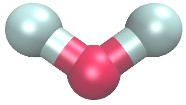
\includegraphics[width=2.4cm]{single_water_LR.jpg}
\caption{
\label{fig:single_water}
Coordinates of a single water molecule in our example.
(Atomic radii not to scale.)
}
\end{figure}

  Here we show an example of a espresso-template file for water.
  %``.et'' files can store topology and force-field settings in raw ESPResSo format.
(The settings shown here are borrowed from the simple-point-charge 
 \cite{Berendsen++StraatsmaJPhysChem1987} SPC/E model.) 
   %and can be overridden or modified by 
   %combining this ET file with other ET files.)
In addition to coordinates, topology and force-field settings, 
``ET'' files can optionally include any other kind of ESPResSo settings
including RATTLE constraints, k-space settings, etc.
\textit{(Unicode is supported.)}
%\pagebreak

\begin{verbatim}
# file "spce_flex.et"
#
#    H1     H2
#      \   /
#        O
#
# This is stiff but flexible version of the "SPC/E" 
# water model that uses short-range electrostatics.
# (Not optimized.  Do not use it in a publication.)

SPCEflex {

  write("Data Atoms") {
    part $atom:o  pos  0.00000 0.000000 0.0000 type @atom:O q -0.8476 mass 16.0 
    part $atom:h1 pos  0.81649 0.577359 0.0000 type @atom:H q  0.4238 mass  1.0
    part $atom:h2 pos -0.81649 0.577359 0.0000 type @atom:H q  0.4238 mass  1.0
  }

  write("Data Bonds") {
    part $atom:o  bond @bond:b_OH  $atom:h1
    part $atom:o  bond @bond:b_OH  $atom:h2
  }

  # 2-body non-bonded interactions:

  write_once("In Settings") {
    inter @atom:O @atom:O lennard-jones 0.1553 3.166 10.0
    inter @atom:O @atom:H lennard-jones 0.0    3.166 10.0
    inter @atom:H @atom:H lennard-jones 0.0    3.166 10.0
  }

  # 2-body (bonded) interactions:
  #
  #   Ubond(r) = (k/2)*(r-r0)^2
  #
  #           bond_type       bond_Style   k     r0
  write_once("In Settings") {
    inter  @bond:b_OH         harmonic    600.0  1.0
  }

  
  # 3-body interactions in this example are of this type:
  #
  # Uangle(theta) = (k/2)*(theta-theta0)^2   
  #
  #     (k in kcal/mol/rad^2, theta0 in radians)
  #
  # inter  angleType  stylename  k     theta0

  write_once("In Settings") {
    inter @bond:a_HOH   angle   600.0 1.91061193216
  }

  write("Data Angles") {
    part $atom:o  bond  @bond:a_HOH  $atom:h1  $atom:h2
  }

} # SPCEflex
\end{verbatim}

\rule{10cm}{0.4mm}

\textit{\textbf{Comment: Currently, in an ``.ET'' file, the TCL commands that describe a molecule must be divided into different sections, such as ``Data Atoms'', ``Data Bonds'', and ``In Settings''  See section \ref{sec:DataIn} for details.}}

\rule{10cm}{0.4mm}

Words which are preceded by ``\$'' or ``@'' characters 
are counter variables and will be replaced by integers. 
(See section \ref{sec:variables} for details.)
Users can include SPCE water in their simulations using commands like these:
\begin{verbatim}
# -- file "system.et" --
import "spce_flex.et"
wat = new SPCE [1000]
\end{verbatim}
You can now use ``emoltemplate.sh'' to create simulation input files for ESPResSo
\begin{verbatim}
emoltemplate.sh -pdb coords.pdb system.et
\end{verbatim}
This command will create espresso input files 
for the molecular system described in ``system.et'',
using the desired atom style (``full'' by default).
In this example, emoltemplate is relying on an external file (``coords.pdb'')
to supply the atomic coordinates of the water molecules, as well as
the periodic boundary conditions.
Coordinates in XYZ format are also supported using ``-xyz coords.xyz''. 


\subsubsection*{\textit{Details}}
\textit{Note that since XYZ files lack boundary information, you must also 
 include a ``Boundary'' section in your ``.et'' file, as demonstrated 
 in section \ref{sec:pbc}. 
 In both cases, the order of the atom types in a PDB or XYZ file 
 (after sorting) should match the order they are created by emoltemplate
 (which is determined by the order of the ``new'' commands 
 in the ET file). 
 Unfortunately this may require careful manual editing of the PDB or XYZ file.}
  %(See appendix \ref{sec:order_customization} for instructions
  % how to customize the order of emoltemplate counting).

\subsection{Coordinate generation}
\label{sec:coords_intro}
It is not necessary to provide a separate file with atomic coordinates. 
It is more common to manually specify the location 
(and orientation) of the molecules in your system using the
 ``.move()'' and ``.rot()'' commands %for rigid-body movement 
in the ET file itself 
(discussed in section \ref{sec:coordinates}).
For example you can replace the line:
\begin{verbatim}
wat = new SPCEflex [1000]
\end{verbatim}
from the example above with 1000 lines:
\begin{verbatim}
wat1    = new SPCEflex
wat2    = new SPCEflex.move(3.450, 0.0, 0.0)
wat3    = new SPCEflex.move(6.900, 0.0, 0.0)
wat4    = new SPCEflex.move(10.35, 0.0, 0.0)
  :           :
wat1000 = new SPCEflex.move(34.50, 34.50, 34.50)
\end{verbatim}
Specifying geometry this way is tedious.
Alternatively, emoltemplate has simple commands for arranging multiple 
copies of a molecule in periodic, crystalline, toroidal, and helical 
1-D, 2-D, and 3-D lattices.  
For example, you can generate a simple cubic lattice of 
10$\times$10$\times$10 water molecules
(with a 3.45 Angstrom spacing)
using a single command 
(which in this example we split into multiple lines)
\begin{verbatim}
wat  = new SPCEflex [10].move(0,0,3.45) 
                    [10].move(0,3.45,0) 
                    [10].move(3.45,0,0)
\end{verbatim}
(See section \ref{sec:coordinates} for more details and examples.)
This will create 1000 molecules with names like
``wat[0][0][0]'', ``wat[0][0][1]'',$\ldots$, ``wat[9][9][9]''.
You can always access individual atomIDs, and bondIDs
(if present), for any molecule 
elsewhere in your ET files using this notation:
``\$atom:wat[2][3][4]/h1''
This allows you to define interactions which link
different molecules together (see section \ref{sec:coordinates}).

A list of available coordinate transformations 
is provided in section \ref{sec:xforms_table}.

%\subsubsection*{Defining the simulation boundary}
\subsubsection*{Boundary Conditions:}
\label{sec:pbc}
ESPResSo simulations have finite volume and are usually periodic. 
We must specify the dimensions of the simulation boundary 
using the ``write\_once(``Data Boundary'')'' command.  
\begin{verbatim}
write_once("Data Boundary") {
  setmd box 34.5 34.5 34.5
  setmd periodic 1 1 1
}
\end{verbatim}
This is usually specified in the outermost ET file 
(``system.et'' in this example).

This system is shown in figure \ref{fig:spce_x_1000}a).
After you have specified the geometry, 
then you can run emoltemplate.sh this way:
\begin{verbatim}
emoltemplate.sh system.et
\end{verbatim}

\begin{figure}[htbp]
\centering
\textbf{a)}
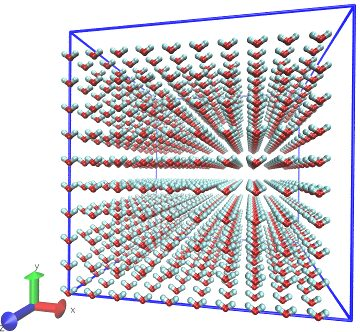
\includegraphics[width=5cm]{waterSPCEx1000_LR.jpg}
\textbf{b)}
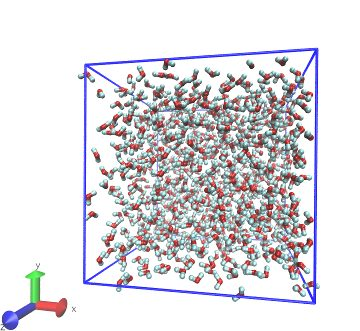
\includegraphics[width=5cm]{waterSPCEx1000_t=25_LR.jpg}
\caption{
\label{fig:spce_x_1000}
A box of 1000 water molecules (before and after pressure equilibration), 
generated by emoltemplate and visualized by VMD.
% with the topotools plugin.
%(The VMD console commands used for visualization were:
%``topo readlammpsdata system.data full'',
%``animate write psf system.psf'',
%``pbc wrap -compound res -all'', and 
%``pbc box''.  See the online examples for details.)
}
\end{figure}

  %\subsubsection*{\textit{Non-periodic simulations}}
  %The use of periodic boundary conditions in ESPResSo is optional.
  %For example the ``boundary p p f'' command turns off 
  %periodic boundary conditions in the Z-direction. 
  %  %When using ESPResSo, commands like this belong 
  %  %near the beginning of a ESPResSo input script.
  %In emoltemplate.sh, these kinds of commands go in the ``In Init'' section:
  %\begin{verbatim}
  %write_once("In Init") {
  %  boundary p p f
  %}
  %\end{verbatim}
  %Note that the simulation volume is still finite.
  %(Currently, as of 2012-10-18, 
  % atoms which escape the simulation boundary are lost/destroyed.)
  %  %(Of course, you can always manually edit the ESPResSo input script 
  %  % file that was generated by emoltemplate.sh before running ESPResSo.
  %  % These files are explained below.)


\subsection{Running a ESPResSo simulation (after using emoltemplate)}
\label{sec:run}
Emoltemplate will create the following file: 
``system.tcl''
This file contains TCL commands 
for creating atoms, bonds, and other interactions in ESPResSo.
They can be run in ESPResSo directly.
  %with minimal modification (see below).

To \textit{run} a simulation, you will have to 
edit this file in order to add additional
commands to tell ESPResSo about the simulation conditions
you want to use (temperature, pressure), 
how long to run the simulation,
how to integrate the equations of motion,
and how to write the results to a file (file format, frequency, etc).
%Emoltemplate.sh can not do this for you.
%Some simple examples (which you can paste into your input script)
%are provided in the 
%\textit{online examples} 
%which can be downloaded from \url{http://moltemplate.org/espresso}.

\pagebreak
\section{Overview}
  %This paragraph below is an excellent
  %summary/explanation of what emoltemplate.sh does.

\subsection{Basics: The \textit{write()} and \textit{write\_once()} commands}
\label{sec:write}
Each ET file typically contains one or more 
``write'' or ``write\_once'' commands. 
These commands have the following syntax 
\begin{verbatim}
write_once(filename) {text_block}
\end{verbatim}
This creates a new file with the desired file name 
and fills it with the text enclosed in curly brackets \{\}.
  %(after any necessary variable substitutions have been made). 
Text blocks usually span multiple lines and contain counter variables 
(beginning with ``@'' or ``\$'').
which are replaced with numbers.
However the ``write()'' command will repeatedly append the 
same block of text to the file every time the molecule 
(in which the write command appears) is generated or copied 
(using the ``new'' command, 
after incrementing the appropriate counters,
as explained in \ref{sec:instance_variables}).
 %incrementing any counter 
 %variables beginning with \$). 
  %When this happens, any counter variables beginning 
  %with \$ will be incremented.)
%On the other hand, ``write\_once()'' commands print their text only once.
%This is useful in certain cases.  For example, there is no need to redundantly 
%specify the mass of the ``O'' and ``H'' atoms every time you create another copy
%of the same molecule. This kind of data should be written only once using the 
%``write\_once(``Data Masses'')'' command.
   %However, new atoms are generated every time a new copy of a previously 
   %defined molecule is created.  This kind of data should be written using the
   %``write(``Data Atoms'')'' command.


\subsection{Basics: counter variables}
\label{sec:variables}

Words following a ``@'' or a ``\$'' character
are \textit{counter variables}. 
By default, 
\textit{all counter variables are substituted with a numeric counter}
before they are written to a file. 
  %(or to a section of a ESPResSo DATA file as 
  %explained in section \ref{sec:write}).
These counters begin at 1 (by default), and 
are incremented as the system size and complexity grows (see below).

These words typically contain a colon (:) followed by more text.
The text preceding this colon is the \textit{category name}. 
(For example: ``\$atom:'', ``@atom:'', ``@bond:''.)
Variables belonging to different categories 
are counted independently. 

Users can override these assignment rules and create custom categories.
(See appendices \ref{sec:manual_assignment} and \ref{sec:custom_categories}
for details.)

\subsubsection{Static counters begin with ``@''}
\label{sec:static_variables}

``@'' variables generally correspond to \textit{types}: 
such as atom types, bond types, angle types, dihedral types, improper types.
These are simple variables and they assigned to unique integers in the 
order they are read from your ET files.
Each uniquely named variable in each category is assigned to a different 
integer.  For example, ``@bond:'' type variables are numbered from ``1''
to the number of \textit{bonded-interaction types}.
Later, ESPResSo will use this integer to lookup the bond-length and Hooke's-law 
elastic constant describing the force between two atoms, and the
angle between three atoms, etc...

%These numbers do not change if the number of molecule copies 
%increases.

\subsubsection{Instance counters begin with ``\$''}
\label{sec:instance_variables}

On the other hand, ``\$'' variables are created whenever a copy 
of a molecule is created (using the ``new'' command).  
(These are usually atom-ID numbers.)
If you create 1000 copies of a water molecule using a command like 
\begin{verbatim}
wat = new SPCEflex[10][10][10]
\end{verbatim}
then emoltemplate creates 3000 ``\$atom'' variables with names like
\begin{verbatim}
$atom:wat[0][0][0]/o
$atom:wat[0][0][0]/h1
$atom:wat[0][0][0]/h2
$atom:wat[0][0][1]/o
$atom:wat[0][0][1]/h1
$atom:wat[0][0][1]/h2
\end{verbatim}
$\quad \vdots $
\begin{verbatim}
$atom:wat[9][9][9]/o
$atom:wat[9][9][9]/h1
$atom:wat[9][9][9]/h2
\end{verbatim}



\subsubsection{Variable names: short-names \textit{vs.} full-names}
\label{sec:full_names}

In the example above, the \$ variables have full-names like
``\$atom:wat[8][3][7]/h1'', not ``\$atom:h1''.  However inside the
definition of the water molecule, you don't specify the full name.
You can refer to this atom as ``\$atom:h1''.
Likewise, the full-name for the @atom variables is actually
``@atom:SPCEflex/H'', not ``@atom:H''. 
However inside the definition of the water molecule,
you typically use the shorthand notation ``@atom:H''.

\subsubsection{Numeric substitution}
Before being written to a file, every variable (either \$ or @) 
with a unique \textit{full-name} will be assigned to a unique integer, 
starting at 1 by default.
  %(You can override this choice if you want to using the ``-a'' flag.)

The various \$atom variables in the water example will be substituted 
with integers from 1 to 3000 (assuming no other molecules are present).
But the ``@atom:O'' and ``@atom:H'' variables
(which are shorthand for ``@atom:SPCEflex/O'' and ``@atom:SPCEflex/H'')
will be assigned to to ``1'' and ``2''
(again, assuming no other molecule types are present).

So, in summary, @ variables increase with the \textit{complexity} 
of your system
(IE the number of molecule types or force-field parameters), 
but \$ variables increase with the \textit{size} of your system.

\subsubsection{Variable scope}
\label{sec:variable_scope}
This effectively means that all variables are specific to
local molecules they were defined in.
In other words, an atom type named ``@atom:H'' inside 
the ``SPCEflex'' molecule, will be assigned to a different number
than an atom named ``@atom:H'' in an ``Arginine'' molecule.
This is because the two variables will have different \textit{full} names
(``@atom:SPCEflex/H'', and ``@atom:Arginine/H'').


\subsubsection*{Sharing atom types or other variables between molecules}
There are several ways to share atom types between two molecules.
The \textit{recommended way} is to define them in a separate
file and refer to them when needed.
This approach is demonstrated in section \ref{sec:2bead}.

\textit{(Alternately, you can define them outside the current molecule definition,
and use file-system-path-like syntax 
(``../'', or ``../../'' or ``/'')
to access atoms (or molecules) outside of the current molecule.
   %(or nested within the definition of another molecule).
For example, two different molecule types can share the same type of
hydrogen atom by referring to it using this syntax: ``@atom:../H''.
  %(Two molecules could share the same atom-id in a similar way, 
  % using ``\$atom:../h1''.  This is not recommended)
For details, see
section \ref{sec:paths}.
and appendix \ref{sec:adv_variable_syntax}.)
  %To be on the safe side, if you want to define a single 
  %hydrogen atom type named ``H'' globally, for example, 
  %then you would refer to this atom everywhere using ``@atom:/H''.
  %(A more portable alternative would be to use the ``@atom:.../H'' 
  % syntax explained in appendix \ref{sec:adv_variable_syntax}.
  % This is similar to ``@atom:/H'',
  % however using the ellipsis syntax ``@atom:.../H'' allows you to 
  % share your molecule definitions (ET files) with others 
  % who may have a different notion of what the ``H'' atom is.)
}



\subsection{Troubleshooting using the \textit{output\_ttree} directory}
\label{sec:output_ttree}
Users can see what numbers were assigned to each variable 
by inspecting the contents of the ``output\_ttree'' subdirectory
created by emoltemplate. 
Unfortunately, it is typical for ESPResSo to crash the first time you 
attempt to run it on a TCL file created by emoltemplate.  This often occurs 
if you failed to spell atom types and other variables consistently.
The ESPResSo error message 
will help you determine what type of mistake you made.
(For example, what type of variable was misspelled or placed in the wrong place?)

To help you, the ``output\_ttree'' directory contains a file named 
``ttree\_assignments.txt''. 
This is a simple 2-column text file containing a list of \textit{all} 
of the variables you have created in one column, and the numbers they
were assigned to in the other column.
(There is also a comment on each line beginning with a ``\#'' character which
indicates the file and line number where this variable is first used.)
This directory also contains all of the files that you created. 
The versions with a ``.template'' extension contain text
interspersed with \textit{full} variable names (before numeric substitution).
(A spelling mistake, like using ``\$atom:h'' when you meant to say ``\$atom:h1''
or ``@atom:H'' will show up in these files if you inspect them carefully.)
This can help you identify where the mistake occurred
in your ET files.

Once a molecular system is debugged and working, users 
can ignore or discard the contents of this directory.


\subsection{``Data'' and ``In''}
\label{sec:DataIn}

All files whose names begin with ``In '' or ``Data '' are special.
The emoltemplate.sh script copies the contents 
of these files into the final TCL file in a different order than the
order the commands were issued.
Text written to ``In Init'' and ``In Settings''
(which usually contain force-field parameters)
%or ``Data Pair Coeffs'',
%``Data Bond Coeffs'',  ``Data Angle Coeffs'', and  ``Data Dihedral Coeffs''
appears in your TCL file before text written to files with names like
``Data Atoms'', ``Data Bonds'', ``Data Angles'',
``Data Dihedrals'', 
``Data Angles By Type'', and
``Data Dihedrals By Type'',
for example.
(These files contain coordinate data, bonds, angles, dihedrals,
as well as rules for generating angles and dihedrals, respectively.
Emoltemplate recognizes these files, and treats them differently.)
Afterwards these files are moved to the ``output\_ttree/'' directory, 
in an effort to clean things up and hide them from view.
(But theese files are not discarded.  If there is an error in your files,
the ``output\_ttree/'' directory is a good place to find it.)
  %Users can also create their own custom sections to a ESPResSo TCL file.
  %(See section \ref{sec:custom_data}.

More generally, the ``write()'' and ``write\_once()'' commands can be used to
create any other files you may need to run your simulations
which refer to the same \textit{@atom} and \textit{@bond} types.
%Files whose names do not begin with ``In '' or ``Data ''
%can have any format
%(and are not moved or cleaned up).
   %(These files are not removed or hidden later.) 
(See section \ref{sec:aux_files} 
  % and \ref{sec:output_ttree} for examples
for an example.)

%\rule{10cm}{0.4mm}
%\textit{(Comment: is because moltemplate was originally designed to create files for LAMMPS.  LAMMPS files are strictly divided into sections such as ``Data Atoms'', ``Data Bonds'', ``In Settings'', etc...  It may seem somewhat arbitrary to organize ESPResSo's TCL files in this way.  The goal was to make it much easier to convert files between LAMMPS(.lt) and ESPResSo(.et) formats.  This could be advantageous since there are many more force-fields and examples which are already available in LAMMPS(.lt) format.  Hopefully they will eventually be converted.)}
%\rule{10cm}{0.4mm}


\subsection{\textit{(Advanced)} 
             Using emoltemplate to generate auxiliary files}
\label{sec:aux_files}
The following excerpt from an ET file 
creates a file named ``table\_XCCX.dat'', containing 
3-column (angle, F, V) data for a tabulated dihedral interaction.
It then refers to this file later on.
\begin{verbatim}
  write_once("table_XCCX.dat") {
    # 12
    0.0000000000000000 -0.8000000000000000  0.3000000000000000
    0.5235987755982988  0.14999999999999997 1.0598076211353318
    1.0471975511965976  1.0598076211353316  0.1500000000000000
    1.5707963267948966  0.2999999999999997  -0.800000000000000
    2.0943951023931953 -0.5401923788646684 -0.15000000000000008
    2.6179938779914944  0.1500000000000005  0.5401923788646684
    3.141592653589793   0.8000000000000000 -0.3000000000000000
    3.665191429188092  -0.1499999999999996 -1.0598076211353318
    4.1887902047863905 -1.0598076211353316 -0.15000000000000047
    4.71238898038469   -0.3000000000000004  0.8000000000000000
    5.235987755982989   0.5401923788646685  0.1500000000000000
    5.759586531581287  -0.14999999999999822 -0.5401923788646685
  }
  write_once("In Settings") {
    inter @bond:xccx tabulated dihedral table_XCCX.dat
  }
  write_once("Data Dihedrals By Type") {
    @bond:xccx @atom:* @atom:C @atom:C @atom:* @bond:* @bond:* @bond:*
  }
\end{verbatim}
  %         Generated with
  % #!/bin/env python
  % from math import *
  % N=12
  % for i in range(0,N):
  %     x = (2*pi*i)/N
  %     print(str(x)+' '+str(0.8*sin(3*(x-pi/6))+0.3*sin(x))+' '+
  %           str(0.8*cos(3*(x-pi/6))+0.3*cos(x)))
As new force-field styles and/or features are added to ESPResSo, 
the files they depend on can be embedded in an ET file in this way. 


  %\subsection{\textit{(Advanced)} Making custom DATA sections}
  %\label{sec:custom_data}
  %Suppose that in the future, a new feature is added to ESPResSo 
  %so that it now becomes necessary to supply a new section named 
  %``Foo Fee Fum'', for example.  You could do that using this command:
  %\begin{verbatim}
  %write_once("Data Foo Fee Fum") {
  %  File contents goes here. (These files can contain
  %  atom counters and/or other counter variables).
  %}
  %\end{verbatim}
  %This way emoltemplate copy this text into the ``Foo Fee Fum'' section at
  %the end of the DATA file it is constructing.
  %This allows users to adapt to future changes in the ESPResSo data file format.


\subsubsection*{Referencing TCL variables \textit{inside} an .ET file:}
\textit{
The \$ character is used to denote \textbf{both} TCL variables
\textbf{and} emoltemplate variables.  Users can include references
to TCL variables in their .ET files, but they must precede these
them with a ``\textbackslash'' character so that emoltemplate does
confuse them with its own.
(For example, to refer to TCL variable \textbf{x} in a write() statement,
you must use \textbf{\textbackslash\$x}, not \textbf{\$x})
}
<<<<<<< HEAD


=======


>>>>>>> 4b707e6d0f50437da86f5740b7386be9af8b960d
\subsubsection*{Does ``@atom:H'' conflict with ``\$atom:H''?}
\label{sec:vardetails}
No.  It is okay for static(@) and instance(\$) variables to share the same names.
(Moltemplate considers them distinct variables and they will be assigned independently.)

\subsubsection*{Addional Details}
Variable and molecule names can include unicode characters.
They can also include some whitespace characters and other special characters
by using backslashes and curly-brackets, for example:
``@\{atom: CA \}'' and ``@atom:\textbackslash\ CA\textbackslash\ ''.
Curly-brackets are useful to clarify when a variable name begins and ends,
such as in this example: ``@\{atom:C\}-@\{atom:H\}''.
(This prevents the ``-'' character from being appended to the end of the 
``C'' variable name.)


\textit{(Unicode is supported.)}



\pagebreak
\section{ Object composition and coordinate generation }
\label{sec:coordinates}


Objects can be connected together to form larger molecule objects.
These objects can be used to form still larger objects.
As an example, we define a small 2-atom molecule named ``Monomer'',
and use it to construct a short polymer (``Peptide'').

\begin{figure}[htbp]
\centering
\textbf{a)}
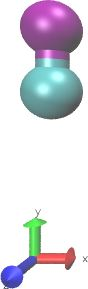
\includegraphics[height=3cm]{2bead_residue.jpg}
\quad \quad \quad \quad \quad
\textbf{b)}
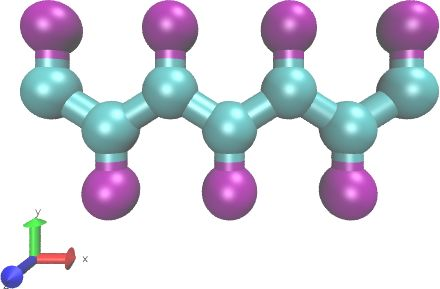
\includegraphics[height=3cm]{2bead_peptide.jpg}
\newline
\vspace{10 mm}
\newline
\textbf{c)}
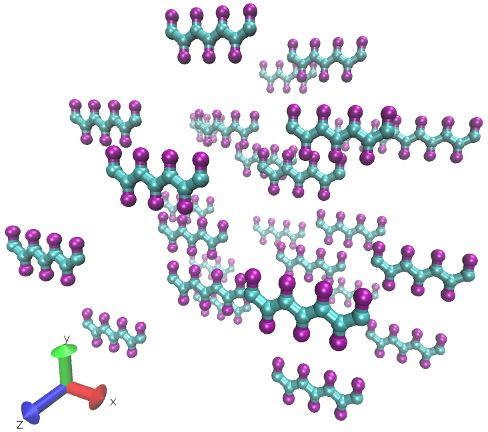
\includegraphics[width=4cm]{2bead_peptides_nopbc_t=0_LR.jpg}
\textbf{d)}
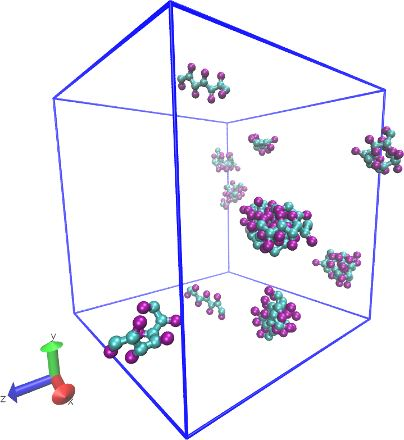
\includegraphics[width=4cm]{2bead_peptides_t=100ps_LR.jpg}
\caption{
\label{fig:2bead_peptide}
\textbf{a)-b)}
\textit{Building a complex system from small pieces:}
Construction of a polymer (\textbf{b}) 
out of smaller (2-atom) subunits (\textbf{a})
using composition and rigid-body transformations. 
Bonds connecting different residues together (blue) 
must be declared explicitly, 
but angle and dihedral interactions will be generated automatically.
See section \ref{sec:2bead} for details.
\textbf{c)}
An irregular lattice of short polymers.
(See section \ref{sec:multidimensional_arrays}.)
\textbf{d)}
The same system after 100000 time steps using Langevin dynamics.
    %the Langevin dynamics settings from section \ref{sec:runcg}.
  %(The VMD console commands used for visualization were:
  %``topo readlammpsdata system.data full'',
  %``animate write psf system.psf'',
  %``pbc wrap -compound res -all'', and 
  %``pbc box''.  See online examples for details.)
}
\end{figure}



\pagebreak

\subsection{Building a large molecule from smaller pieces}
\label{sec:2bead}

\begin{verbatim}
# -- file "monomer.et" --

import "forcefield.et"   # contains force-field parameters

Monomer inherits ForceField {
  write("Data Atoms") {
    part $atom:ca  pos 0.000 1.000 0.000  type @atom:CA  q 0.0  mass 13.0 
    part $atom:r   pos 0.000 4.400 0.000  type @atom:R   q 0.0  mass 50.0
  }
  write("Data Bonds") {
    part $atom:ca bond @bond:b_Sidechain $atom:r
  }
}
\end{verbatim}



In this example we will define two kinds of molecule objects:
``Monomer'', and ``Peptide'' (\textit{defined later}).
It is often convenient to store atom types, masses, and force-field 
parameters in a separate file so that they
can be shared between these different molecules.
We do that in the ``forcefield.lt'' file below:


\begin{verbatim}
# -- file "forcefield.et" --

ForceField {

  # There are 2 atom types: "CA" and "R"

  # 2-body non-bonded interactions:
  #
  #   Uij(r) = 4*eps_ij * ( (sig_ij/r)^12 - (sig_ij/r)^6 )
  #
  #            i        j          stylename     eps   sig  rcut
  #
  write_once("In Settings") {
    inter   @atom:CA  @atom:CA   lennard-jones  0.10   2.0  9.0
    inter   @atom:R   @atom:R    lennard-jones  0.50   3.6  9.0
    inter   @atom:CA  @atom:R    lennard-jones  0.2236 2.8  9.0
  }

  # 2-body (bonded) interactions:
  #
  #   Ubond(r) = (k/2)*(r-r0)^2
  #
  #          bond_type       bond_Style    k      r0
  write_once("In Settings") {
    inter  @bond:b_Sidechain  harmonic    30.0   3.4
    inter  @bond:b_Backbone   harmonic    30.0   3.7
  }

  # Although the simple "Monomer" object we defined above has only
  # two atoms, later on, we will create molecules with many bonds.
  # By convention, in this file we keep track of all of the possible
  # interactions which could exist between these atoms:

  # 3-body interactions in this example are listed by atomType and bondType
  # Rules for determining 3-body angle interactions by type
  # angle-type     atomType1 atomType2 atomType3  bondType1 bondType2

  write_once("Data Angles By Type") {
    @bond:a_Backbone  @atom:CA @atom:CA  @atom:CA     *        *
    @bond:a_Sidechain @atom:CA @atom:CA  @atom:R      *        *
  }

  # Uangle(theta) = (k/2)*(theta-theta0)^2   
  #     (k in kcal/mol/rad^2, theta0 in radians)
  #
  # The corresponding command is:
  #
  #          angleType        angle    k     theta0

  write_once("In Settings") {
    inter  @bond:a_Sidechain  angle   30.0   1.9896753  #114 degrees
    inter  @bond:a_Backbone   angle   30.0   2.3038346  #132 degrees
  }

  # Rules for determining 4-body dihedral interactions by type
  # dihedralType atmType1 atmType2 atmType3 atmType4  bondType1 bnd2 bnd3

  write_once("Data Dihedrals By Type") {
    @bond:d_CCCC @atom:CA @atom:CA @atom:CA @atom:CA      *     *    *
    @bond:d_RCCR @atom:R  @atom:CA @atom:CA @atom:R       *     *    *
  }

  # 4-body interactions in this example are listed by atomType
  # The forumula used is:
  #
  # Udihedral(phi) = K * (1 + cos(n*phi - d))
  #
  #     The d parameter is in radians, K is in kcal/mol/rad^2.
  #
  # The corresponding command is 
  # inter  dihedralType    dihedral       K  n  d

  write_once("In Settings") {
    inter  @bond:d_CCCC    dihedral     -0.5 1 3.141592653589793
    inter  @bond:d_RCCR    dihedral     -1.5 1 3.141592653589793
  }

} # ForceField
\end{verbatim}

\subsubsection{Building a simple polymer}
We construct a short polymer by making 7 copies of ``Monomer'',
rotating and moving each copy:
\label{sec:2beadPeptide}
\begin{verbatim}
# -- file "peptide.et" --

import "monomer.et"

Peptide inherits ForceField {
  res1 = new Monomer
  res2 = new Monomer.rot(180.0, 1,0,0).move(3.2,0,0)
  res3 = new Monomer.rot(360.0, 1,0,0).move(6.4,0,0)
  res4 = new Monomer.rot(540.0, 1,0,0).move(9.6,0,0)
  res5 = new Monomer.rot(720.0, 1,0,0).move(12.8,0,0)
  res6 = new Monomer.rot(900.0, 1,0,0).move(16.0,0,0)
  res7 = new Monomer.rot(1080.0, 1,0,0).move(19.2,0,0)

  # Now, link the residues together this way:
  write("Data Bonds") {
    part  $atom:res1/ca  bond @bond:b_Backbone  $atom:res2/ca
    part  $atom:res2/ca  bond @bond:b_Backbone  $atom:res3/ca
    part  $atom:res3/ca  bond @bond:b_Backbone  $atom:res4/ca
    part  $atom:res4/ca  bond @bond:b_Backbone  $atom:res5/ca
    part  $atom:res5/ca  bond @bond:b_Backbone  $atom:res6/ca
    part  $atom:res6/ca  bond @bond:b_Backbone  $atom:res7/ca
  }
}
\end{verbatim}
The position and orientation of each copy of ``Monomer'' 
is specified after the ``new'' statement. 
Each ``new'' statement is typically followed by a chain of 
move/rotate/scale functions separated by dots, evaluated left-to-right
(optionally followed by square brackets and then more dots). 
For example, ``res2'' is a copy of ``Monomer'' which is first rotated 
180 degrees around the X axis (denoted by ``1,0,0''), 
and \textbf{then} moved in the (3.2,0,0) direction.
(The last three arguments to the ``rot()'' command 
 denote the axis of rotation, which does not have to be normalized.)
(A list of available coordinate transformations 
is provided in section \ref{sec:xforms_table}.)

\textit{(Note: Although we did not do this here, 
it is sometimes convenient to represent polymers as 1-dimensional arrays. 
See sections \ref{sec:arrays} and \ref{sec:random_arrays} for examples.)}

To bond atoms in different molecules or molecular subunits together, we used 
the write(``Data Bonds'') command to append additional bonds to the system.



%\subsubsection{Sharing atom, bond and angle types}
%Normally you must separately define the parameters for all of the atoms types,
%and bond types, angle types etc... in every type of molecule.
%However different kinds of monomers in a heteropolymer typically will 
%share some common backbone atom types and other properties.
%You must be careful to indicate which atom and bond types are shared between
%different monomers by referring them using a ``../'' prefix.
%(See sections \ref{sec:variable_scope}, 
%\ref{sec:paths}, and 
%\ref{sec:butane} for details and examples.)
%\textit{Note: There is a heteropolymer example in the the 
%``Monomer\_heteropolymer/'' directory in the online examples.
%This example demonstrates how to share backbone atoms, bonds, and angles. 
%You can also define specific angle or dihedral interactions which are
%specific to the atom types in different residues.}


\subsection{Bonded interactions \textit{by type}}
\label{sec:nbody_by_type_intro}

In this example we did \textit{not} provide a list of all 3-body
and 4-body forces between bonded atoms in the polymer.
(for example using the ``write\_once("Data Angles")'' command
from section \ref{sec:spce_example},
\textit{or} 
the ``write\_once("Data Dihedrals")'' command)
Instead we provided emoltemplate.sh with instructions to help it figure out 
which atoms participate in 3-body and 4-body bonded interactions.
Emoltemplate can detect consecutively bonded atoms and 
determine the forces between them based on atom type.
(Bond type can also be used as a criteria.)
We did this in ``forcefield.et'' using the
\mbox{``write\_once("Data Angles By Type")''} and 
\mbox{``write\_once("Data Dihedrals By Type")''} 
commands.
%You can also generate improper interactions 
%between any 4-atoms bonded together in a T-shaped topology
%using the  ``write\_once("Impropers By Type")'' command.
%See appendix \ref{sec:nbody_by_type} for more details.
\textit{(More general interactions are possible.
 See appendix \ref{sec:nbody_by_type_custom}.)}

  %\subsubsection*{\textit{(Advanced)} Order matters when sets overlap}
  %Bonded-interactions are generated in the order they appear in the ET file.
  %Interactions which are declared later may override the settings of 
  %interactions which appear earlier, such as in this example:
  %\begin{verbatim}
  %  write_once("Data Angles By Type") {
  %    @bond:a_Backbone  @atom:C* @atom:C*  @atom:*    @bond:*   @bond:*
  %    @bond:a_Sidechain @atom:CA @atom:CA  @atom:R    @bond:*   @bond:*
  %  }
  %\end{verbatim}
  % %Here the first line of this file creates a 3-body angle interaction
  % %of type ``@bond:backbone'' between \textit{every} triplet of bonded atoms 
  % %in the molecule whose first two atom types begin with the letter ``C''.
  %The second line creates 3body interactions (of type ``@bond:a_Sidechain'')
  %specifically between atoms of type ``@atom:CA'', ``@atom:CA'', and 
  %``@atom:R'', overriding any triplets of this type which appeared earlier.



%\subsection*{\textit{(Advanced)} Mixing regular and ``By Type'' interactions}

%If an ET file contains both ``Data Angles'' and ``Data Angles By Type'',
%then the interactions explicitly defined in the ``Data Angles'' section will 
%always override the assignments made in ``Data Angles By Type''.
%The also applies to Dihedrals and Impropers.

  %\begin{verbatim}
  %write("Data Angles") {
  %  part $atom:c1 @bond:CCCgeneral $atom:c2 $atom:c3
  %  part $atom:c2 @bond:CCCgeneral $atom:c3 $atom:c4
  %}
  %\end{verbatim}


\section{Arrays and coordinate transformations}
\label{sec:arrays}
Emoltemplate supports 1-dimensional, and multi-dimensional arrays.
These can be used to create straight (or helical) polymers
sheets, tubes, torii.
They are also to fill solid 3-dimensional volumes
with molecules or atoms.
(See sections \ref{sec:coords_intro} and \ref{sec:multidimensional_arrays}.)

Here we show an easier way to create the short polymer 
shown in section \ref{sec:MonomerPeptide}.
You can make 7 copies of the \textit{Monomer} molecule this way:
\begin{verbatim}
  res = new Monomer[7]
\end{verbatim}
This creates 7 new \textit{Monomer} molecules (named 
\mbox{\textit{res[0]}}, 
\mbox{\textit{res[1]}}, 
\mbox{\textit{res[2]}}, 
\mbox{\textit{res[3]}}, ... 
\mbox{\textit{res[6]}}).
Unfortunately, by default, the coordinates of each molecule are identical.
To prevent the atom coordinates from overlapping, you have several choices:

\subsection{Transformations following brackets [] in a new statement}
\label{sec:arrays+xform}
   After every square-bracket [] in a new command,
you can specify a list of transformations to apply.
For example, we could have generated atomic coordinates for the 
the short polymer in section \ref{sec:MonomerPeptide}
using this command:
\begin{verbatim}
  res = new Monomer [7].rot(180, 1,0,0).move(3.2,0,0)
\end{verbatim}
This will create 7 molecules.  
The coordinates of the first molecule \textit{res[0]} are will be unmodified.
However each successive molecule will have its coordinates cumulatively
modified by the commands ``rot(180, 1,0,0)'' followed by ``move(3.2,0,0)''.
\subsubsection*{optional: initial customizations (preceding [] brackets)}
\label{sec:xform+arrays+xform}
You can also make adjustments to the initial coordinates of the molecule
before it is copied, and before any of the array transformations are applied.
For example:
\begin{verbatim}
  res = new Monomer.scale(1.5) [7].rot(180, 1,0,0).move(3.2,0,0)
\end{verbatim}
In this example, the ``scale(1.5)'' transformation is applied once to 
enlarge every \textit{Monomer} monomer initially.
This will happen before any of the rotation and move commands 
are applied to build the polymer
(so the 3.2 Angstrom spacings between each monomer will not be effected).

\subsection{Transformations following instantiation}
\label{sec:xform_after_instance}
Alternately you apply transformations to a molecule 
after they have been created (even if they are part of an array).
\begin{verbatim}
  res = new Monomer [7]

  # Again, the first line creates the molecules named 
  # "res[0]", "res[1]", "res[2]", "res[3]", ... "res[6]".
  # The following lines move them into position.
  res[1].rot(180.0, 1,0,0).move(3.2,0,0)
  res[2].rot(360.0, 1,0,0).move(6.4,0,0)
  res[3].rot(540.0, 1,0,0).move(9.6,0,0)
  res[4].rot(720.0, 1,0,0).move(12.8,0,0)
  res[5].rot(900.0, 1,0,0).move(16.0,0,0)
  res[6].rot(1080.0, 1,0,0).move(19.2,0,0)
\end{verbatim}

\subsection{Transformation order (general case)}
\label{sec:xform_order}
A typical array of molecules might be instantiated this way:
\begin{verbatim}
mols = new Molecule.XFORMS1() [N].XFORMS2()
mols[*].XFORMS3()
\end{verbatim}
The list of transformations denoted by ``XFORMS1'' in this example
are applied to the molecule first.
Then the transformations in ``XFORMS2'' are then applied to each
copy of the molecule multiple times.  
(For the molecule with index ``$i$'', named ``Molecule[$i$]'',
XFORMS2 will be applied $i$ times.)
Finally after all the molecules have been created, the list
of transformations in XFORMS3 will be applied.
For example, to create a ring of 10 peptides of radius 30.0, 
centered at position (0,25,0), use this notation:
\begin{verbatim}
peptide_ring = new Peptide.move(0,30,0) [10].rot(36,1,0,0)
  # After creating it, we can move the entire ring 
  # (These commands are applied last.)
peptide_ring[*].move(0,25,0)
\end{verbatim}


\subsection{Random arrays}
\label{sec:random_arrays}

\begin{figure}[htbp]
\centering
\textbf{a)}

\includegraphics[height=1.2cm]{random_2bead.jpg}
\hspace{0.2cm}
\textbf{b)}
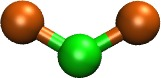
\includegraphics[height=0.75cm]{random_3bead.jpg}
\hspace{0.2cm}
\textbf{c)}
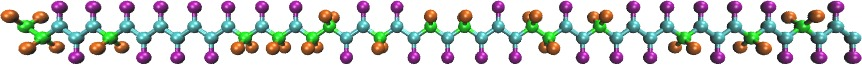
\includegraphics[width=8cm]{random_heteropolymer.jpg}
%\newline
%\vspace{10 mm}
%\newline
\caption{
\label{fig:random_heteropolymer}
A random heteropolymer (\textbf{c}),
composed of of \textit{2bead} and \textit{Monomer3} monomers
(\textbf{a} and \textbf{b}) in a 3:2 ratio.
}
\end{figure}
Arrays of random molecules can be generated using the 
\mbox{\textit{new random() []}} syntax.  For example,
below we define a random polymer composed of 50 
\textit{2bead} and \textit{Monomer3} monomers.
(See figure \ref{fig:random_heteropolymer}.)
\begin{verbatim}
RandPoly50 inherits ForceField {
  # Make a chain of randomly chosen monomers:

  monomers = new random([Monomer, Monomer3], [0.6, 0.4], 123456)
                 [50].rot(180,1,0,0).move(2.95, 0, 0)

  # Now, link the monomers together this way:
  write("Data Bonds") {
    part  $atom:monomers[0]/ca  bond @bond:b_Backbone  $atom:monomers[1]/ca
    part  $atom:monomers[1]/ca  bond @bond:b_Backbone  $atom:monomers[2]/ca
    part  $atom:monomers[2]/ca  bond @bond:b_Backbone  $atom:monomers[3]/ca
    part  $atom:monomers[3]/ca  bond @bond:b_Backbone  $atom:monomers[4]/ca
\end{verbatim}
$\quad \quad \quad \vdots $
%           :           :              :                     :
\begin{verbatim}
    part  $atom:monomers[48]/ca  bond @bond:b_Backbone  $atom:monomers[49]/ca
  }
  #(Note: Both the "Monomer" and "Monomer3" molecules contain atoms
  #       named "$atom:ca".  The atom types are different, however.)
} #RandPoly50
\end{verbatim}
It is also possible to fill a 2 or 3-dimensional volume with
molecules randomly.  This is discussed in section
\ref{sec:random_advanced}.

The \mbox{\textit{new random()}} function takes 2 or 3 arguments:
a list of molecule types 
(\mbox{\textit{Monomer}} and \mbox{\textit{Monomer3}} in this example),
and a list of probabilities (\textit{0.6} and \textit{0.4})
both enclosed in square-brackets [].
There is no limit to the number of molecule types which appear in these lists.
(These lists can also contain vacancies/blanks.
 See section \ref{sec:random_vacancies}.)
(An optional random-seed argument can also be included.
 For example the \mbox{\textit{``123456''}} shown above.
 If you omit this number, then you will get different 
 results each time you run emoltemplate.)
Note that once a molecule containing random monomers is defined, 
(\mbox{\textit{``RandPoly50''}} in this example), each copy of that molecule 
(created using the \textit{new} command) is identical.
\subsubsection*{optional: initial customizations (within \textit{random()})}
As before, you may apply an initial transformation to each monomer type
immediately after its name. 
For example to move the two monomer types 
closer or further away from the polymer axis, you can use:
\begin{verbatim}
  monomers = new random([Monomer.move(0,0.01,0),
                         Monomer3.move(0,-0.01,0)], 
                        ...
\end{verbatim}
These \mbox{\textit{move(0,0.01,0)}} and \mbox{\textit{move(0,-0.01,0)}}
commands will be applied \textit{before} 
the other rotate and move commands are applied
which generate the polymer.

\subsection{[*] and [i-j] notation}
\label{sec:array_wildcards_intro}
You can move the entire array of molecules using ``[*]'' notation:
\begin{verbatim}
  res[*].move(0,0,40)
\end{verbatim}
(Note that ``res.move(0,0,40)'' does not work.
 You must include the ``[*]''.)
You can also use range limits to move only some of the residues:
\begin{verbatim}
  res[2-4].move(0,0,40)
\end{verbatim}
This will move only the third, fourth, and fifth residues.

Of course, as mentioned earlier, you can also always load atom 
coordinates from an external PDB or XYZ file.
Such files can be generated by PACKMOL, 
or a variety of advanced graphical molecular modeling programs. 
For complex systems, this may be the best choice.






\section{Customizing molecule position and topology}
\label{sec:custom_xform}
By default, each copy of a molecule created using the \textit{new}
command is identical.  This need not be the case.

As discussed in section \ref{sec:xform_after_instance},
individual molecules which were recently created
can be moved, rotated, and scaled.
You can also overwrite or delete individual atoms, 
bonds, and other interactions within a molecule, or their subunits.
(See sections 
\ref{sec:delete_atoms_bonds}, 
\ref{sec:custom_atom}, and \ref{sec:adding_atoms_bonds}.)
You make any of these modifications to \textit{some} copies 
of the molecule without effecting other copies.
Furthermore, if those molecules are compound objects 
(if they contain individual molecular subunits within them),
then you can rearrange the positions of their subunits as well.
And all of this can be done from anywhere else in the ET file.
  %\textit{(The notation in section \ref{sec:paths} explains
  %         how to navigate the object hierarchy.)}

For example, suppose we used the ``Peptide'' molecule we defined above
to create a larger, more complex ``Dimer'' molecule.
\begin{verbatim}
Dimer inherits ForceField {
  peptides = new Peptide [2].rot(180,1,0,0).move(0, 12.4, 0)
}
dimer = new Dimer
\end{verbatim}
The \textit{Dimer} molecule is shown in figure \ref{fig:dimers}a). 
\textit{(Note: The rot() and move() commands are only applied to the
the second peptide, as explained in section \ref{sec:arrays+xform}.)}
We can customize the position of the 3rd residue of the second peptide this way:
\begin{verbatim}
dimer/peptide[1]/res[2].move(0,0.2,0.6)
\end{verbatim}
This does not effect the position of \textit{res[2]} in \textit{peptide[0]}
(or in any other \textit{``Peptide''} molecule).
If you want to move them both, you could use a wildcard character ``*''
\begin{verbatim}
dimer/peptide[*]/res[2].move(0,0.2,0.6)
\end{verbatim}
(You an also use ranged notation, such as ``peptide[0-1]'',
 as an alternative to ``peptide[*]''. 
See section \ref{sec:array_wildcards_intro}.
You could also modify the definition of the ``Peptide'' molecule.  
See section \ref{sec:molecule_customization}.)

\subsection{Customizing individual atom locations}
\label{sec:custom_atom}
To customize the positions of \textit{individual atoms}, 
don't use the ``move'' or ``rot'' commands.
Instead simply overwrite their coordinates this way:
 %part $atom:dimer/peptide[0]/res[2]/CA  pos 6.4 8.0 0.0
\begin{verbatim}
write("Data Atoms") {
  part $atom:dimer/peptide[0]/res[2]/ca  pos 6.4 8.2 0.6
}
\end{verbatim}

\subsection{Adding bonds and angles to individual molecules}
\label{sec:adding_atoms_bonds}
Adding additional bonds within a molecule can be accomplished
by writing additional lines of text to the ``Data Bonds'' section.
(This is what we did when we added bonds between residues to create a polymer
 in section \ref{sec:2beadPeptide}.)
Again, bonds and atom names must be referred to by their \textit{full} names.
Bonds and bonded interactions can be deleted using the ``delete'' command.
(See section \ref{sec:delete}.)


\subsection{The \textbf{delete} command}
\label{sec:delete}

\subsubsection{Deleting molecules or molecular subunits}
Molecules can be further customized by deleting 
individual atoms, bonds, bonded-interactions, and entire subunits.
We can \textbf{delete} the 3rd residue of the second peptide, 
use the ``delete'' command:
\begin{verbatim}
delete dimer/peptide[1]/res[2]
\end{verbatim}

\subsubsection{Deleting atoms}
\label{sec:delete_atoms_bonds}
Individual atoms or bonds can be deleted in a similar way:
\begin{verbatim}
delete dimer/peptide[0]/res[3]/ca #<-deletes $atom:ca in dimer/peptide[0]/res[3]
delete dimer/peptide[1]/res[4]/r  #<-deletes $atom:r  in dimer/peptide[1]/res[4]
\end{verbatim}
Whenever an atom or a molecule is deleted, the bonds, angles, dihedrals, 
and improper interactions involving those atoms are deleted as well.
\textit{(In fact, any lines of text in any ``write()'' statement 
containing references to deleted atoms are omitted.)}

Multiple molecules or atoms can moved or deleted in a single command.
For example,
the following command deletes the third, fourth, fifth residues from 
both peptide[0] and peptide[1]:
\begin{verbatim}
delete dimer/peptide[*]/res[2-4]
\end{verbatim}
See section \ref{sec:array_wildcards_intro} for an
explanation of ranged (``[2-4]'') array notation, 
and wildcard characters (``*'').


  %\subsubsection*{The context() modifier.}
  %\textit{THIS FEATURE DOES NOT WORK YET AS OF 2012-10}
  %By default, this transformations is applied relative
  %to the coordinate system in which the command was given.
  %In other words, this command will move the third 
  %residue of peptide[1] in the +Y direction 
  %regardless of the direction that the molecule ``res[2]'' is facing.
  %Alternately, if we want to apply this transformation 
  %in peptide[1]'s local coordinate system, 
  %we would use the context(peptide[1]) command:
  %\begin{verbatim}
  %dimer2/peptide[1]/res[2].context(peptide[1]).move(0,1,0)
  %\end{verbatim}


%\subsubsection*{Examples using center-of-mass coordinate transformations}
%\textit{WARNING: experimental feature 2012-10-18}
%
%You can also center a molecule around it's center-of-mass using ``movecm()'',
%rotate it, and then move it this way:
%\begin{verbatim}
%re6s = new Monomer.movecm(0,0,0).rot(180.0, 1,0,0).move(14.2, 0, 0)
%\end{verbatim}
%By default all rotations are about the origin, not the center-of-mass.
%You can also rotate a molecule around it's center-of-mass using ``rotcm()''
%(without centering it first), and them move the molecule this way:
%\begin{verbatim}
%res6 = new Monomer.rotcm(180.0, 1,0,0).move(14.2, 0, 0)
%\end{verbatim}




\section{Multidimensional arrays}
\label{sec:multidimensional_arrays}
The same techniques work with multidimensional arrays.
Coordinate transformations can be applied to each layer
in a multi-dimensional array.
For example, to create a cubic lattice of 3x3x3 peptides:
you would use this syntax:
\begin{verbatim}
peptides = new Peptide [3].move(0, 0, 30.0)
                       [3].move(0, 30.0, 0)
                       [3].move(30.0, 0, 0)
\end{verbatim}
(Similar commands can be used with rotations to generate objects
with cylindrical, helical, conical, or toroidal symmetry.)

\subsection{Customizing individual rows, columns, or layers}
Similarly, you can customize the position of individual peptides, 
or layers or columns using the methods above:
\begin{verbatim}
peptides[1][*][*].move(20,0,0)
peptides[*][1][*].move(0,0,20)
peptides[*][*][1].move(0,20,0)
\end{verbatim}
(See figure \ref{fig:2bead_peptide}c))

\subsection{Creating random mixtures using multidimensional arrays}
\label{sec:random_advanced}
You can use \mbox{\textit{``new random()''}} to fill space with
a random mixture of molecules.  The following 2-dimensional example
creates a lipid bilayer (shown in figure \ref{fig:random_bilayer})
composed of an equal mixture of 
DPPC and DLPC lipids. (...Whose definition we omit here.  
See the online examples for details.)
\begin{verbatim}
import "lipids"                                     # define DPPC & DLPC
lipids = new random([DPPC,DLPC], [0.5,0.5], 123)    # "123"=random_seed
                    [19].move(7.5,    0,     0)     # lattice spacing 7.5
                    [22].move(3.75, 6.49519, 0)     # hexagonal lattice
                     [2].rot(180, 1, 0, 0)          # 2 monolayers
\end{verbatim}
\begin{figure}[htbp]
\centering
\textbf{a)}
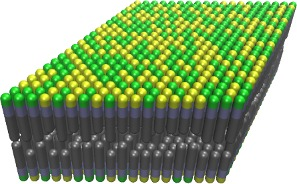
\includegraphics[width=5cm]{lipid_bilayer_mixture_LR.jpg}
\hspace{0.5cm}
\textbf{b)}
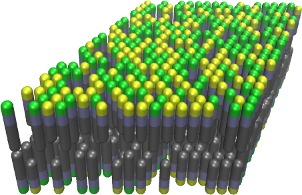
\includegraphics[width=5cm]{lipid_bilayer_vacancies_LR.jpg}
%\newline
%\vspace{10 mm}
%\newline
\caption{
\label{fig:random_bilayer}
A lipid bilayer membrane composed of a random equal mixture of
two different lipid types in a 1:1 ratio.
(See section \ref{sec:random_advanced}.)
In \textbf{b)} one of the molecule types was left blank
leaving vacancies behind.  
(See section \ref{sec:random_vacancies}.)
}
\end{figure}
\subsection{Inserting random vacancies}
\label{sec:random_vacancies}
The list of molecule types passed to the \mbox{\textit{random()}} function
may contain blanks.  In the next example, 30\% of the lipids are missing:
\begin{verbatim}
lipids = new random([DPPC, ,DLPC], [0.35,0.3,0.35], 123) # 2nd element is blank
                    [19].move(7.5,    0,     0)
                    [22].move(3.75, 6.49519, 0)
                     [2].rot(180, 1, 0, 0)     
\end{verbatim}
The results are shown in figure \ref{fig:random_bilayer}b).
\textit{(Note: When this happens, the array will contain missing elements.
 Any attempt to access the atoms inside these missing molecules will
 generate an error message, 
 however moving or deleting array entries 
 using [*] or [i-j] notation should be safe.)}

\subsection{Cutting rectangular holes using \textbf{delete}}
\label{sec:delete_holes}
The delete command can be used to cut large holes in 
1, 2, and 3-dimensional objects.
For example, consider a simple 3-dimensional array of molecules:
\begin{verbatim}
molecules = new OneAtomMolecule [12].move(3.0,0,0)
                                [12].move(0,3.0,0)
                                [12].move(0,0,3.0)
\end{verbatim}
\begin{verbatim}
delete molecules[*][*][2]      
delete molecules[*][*][8]      
delete molecules[6-7][0-8][5-6]
\end{verbatim}
The result of these operations is shown in figure
\ref{fig:delete_holes}.
\textit{(Note: You may move or delete previously deleted array elements
         more than once, and/or deleting overlapping rectangular regions
         without error.)}

\begin{figure}[htbp]
\centering
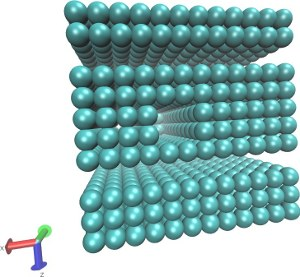
\includegraphics[width=4.0cm]{delete_holes1.jpg}
\caption{
\label{fig:delete_holes}
Rectangular holes can be carved out of an array of molecules
(represented here by blue spheres)
using the ``delete'' command.  Three delete commands were used to
remove the two planar regions and the rectangular hole in the center.
}
\end{figure}





\section{Customizing molecule \textit{types}}
\label{sec:molecule_customization}
You can create modified versions of existing molecule \textit{types}, 
without having to redefine the entire molecule. For example:
\begin{verbatim}
Dimer0 = Dimer.move(-9.6,-6.2, 0).scale(0.3125)
\end{verbatim}
or equivalently:
\begin{verbatim}
Dimer0 = Dimer
Dimer0.move(-9.6,-6.2, 0).scale(0.3125)
\end{verbatim}
This creates a new type of molecule named ``Dimer0'' whose 
coordinates have been centered and rescaled.
(Note that the ``scale()'' command only effects the atomic coordinates.
(You will have to override earlier force field settings,
such as atomic radii and bond-lengths in order for this to work properly.)
If we want to make additional customizations
(such as adding atoms, bonds, or molecular subunits), we could use this syntax:
\begin{verbatim}
Dimer0 = Dimer

# Add some new atoms connecting the two peptides in the dimer

Dimer0 inherits ForceField {
  write("Data Atoms") {
    part $atom:t1  pos  23.0  0.0   0.0  type @atom:CA  q 0.0  mass 13.0
    part $atom:t2  pos  24.7  4.0   0.0  type @atom:CA  q 0.0  mass 13.0
    part $atom:t3  pos  24.7  8.4   0.0  type @atom:CA  q 0.0  mass 13.0
    part $atom:t4  pos  23.0  12.4  0.0  type @atom:CA  q 0.0  mass 13.0
  }
  write("Data Bonds") {
    part $atom:peptides[0]/res7/CA  bond @bond:b_Backbone  $atom:t1
    part $atom:t1      bond @bond:b_Backbone  $atom:t2
    part $atom:t2      bond @bond:b_Backbone  $atom:t3
    part $atom:t3      bond @bond:b_Backbone  $atom:t4
    part $atom:t4      bond @bond:b_Backbone  $atom:peptides[1]/res7/ca
  }
}

# Center and rescale the atoms in all "Dimer0"
Dimer0.move(-9.6,-6.2, 0).scale(0.3125)
\end{verbatim}
The result of these modifications is shown in figure \ref{fig:dimers}b).
\begin{figure}[htbp]
\centering
\textbf{a)}
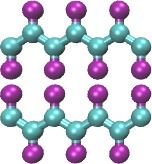
\includegraphics[height=3cm]{dimer_LR.jpg}
\hspace{1cm}
\textbf{b)}
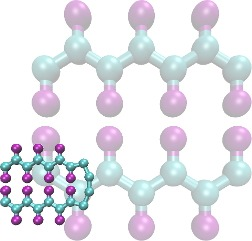
\includegraphics[height=3cm]{dimer+dimer0_transparent_LR.jpg}
%\newline
%\vspace{10 mm}
%\newline
\caption{
\label{fig:dimers}
\textbf{a)}
The ``Dimer'' molecule.  This is a contrived example consisting of
two ``Peptides''.  See section \ref{sec:2beadPeptide}
\textbf{b)}
A customized version of the ``Dimer'' molecule.  
(The original ``Dimer'' is shown faded in the background for comparison.)
}
\end{figure}

\textit{Note1: Coordinate transformations applied to entire
molecule types are an experimental feature as of 2012-10-18.
This feature has not been rigorously tested.}

\textit{Note2: These coordinate transformations will be 
applied \textbf{after} the molecule is completely constructed,
(If you add atoms to the molecule, these will be added before
the coordinate transformations are applied,
even if you issue the command later.)
Consequently, to make things clear, 
I recommend placing the coordinate transforms applied to 
an entire molecule type \textbf{after} all of its internal details 
(bonds, atoms, subunits) have been declared, as we did here.}

\textit{Note3: You may also want all of the atoms in ``Dimer0'' to share the 
 same molecule-ID counter (``\$mol''), so that ESPResSo realizes they belong to 
 the same molecule.  To do that you should delete the 
 \mbox{\textit{``create\_var \{\$mol:.\}''}} line from
 the definition of the Peptide molecule, and add it to \textit{Dimer0}.}

\subsubsection*{\textit{(Advanced)} Inheritance}
\label{sec:inheritance_intro}
The \textit{Dimer0} molecule is a type of \textit{Dimer} molecule.
For those who are familiar with programming, 
relationships like this are analogous to the relationship 
between parent and child objects in an object-oriented programming language.
  %What we have done is equivalent to saying that
  %\textit{Dimer0} inherits from \textit{Dimer}.
More general kinds of inheritance are supported by emoltemplate
and are discussed in section \ref{sec:inheritance}.

\subsubsection*{\textit{(Advanced)} Multiple Inheritance}
If we wanted, we could have created a new molecule type 
(like \textit{``Dimer0''}) 
which includes atom types and features from 
\textit{multiple} different types of molecules.
Section \ref{sec:inheritance} mentions one way to do this
and section \ref{sec:inheritance_vs_object_composition}
discusses alternate approaches.



\section*{Advanced emoltemplate usage}



\subsection{Nesting}
\label{sec:nesting}
Molecule names such as ``Solvent'' (or even ``Water'')
are short and easy to type, but are vague and are not portable.
If you use common, generic molecule names, you will not be able
to combine your molecule templates with templates written 
by others (without carefully checking for naming conflicts).
ET files were meant to be used for storing 
and exchanging libraries of different molecule types.

Suppose, for example, that you want to run a simulation consisting of
different molecule types, each of which belong to different ET files.
Suppose two of the ET files both happen to contain definitions for
``Water''.
Emoltemplate does not detect these name clashes automatically 
and instead attempts to merge the two versions of ``Water'' together,
(most likely creating a molecule with 6 atoms instead of 3).
This is presumably not what you want.

As the number of molecule types grows, 
the possibility of naming clashes increases. 
As the behavior of the same molecule can be approximated 
using many different force fields, 
one has to be careful to avoid clashing molecule names.

To alleviate the problem, you can ``nest'' your 
molecules inside the definition of other molecules or objects.
This reduces the scope in which your molecule is defined.
See section \ref{sec:butane} for an example.


\subsection{A simple force-field example}
Force-field parameters can be shared by groups of related molecules.
In the example below, we create an object named ``TraPPE''.
Later we use it to define a new molecule named ``Cyclopentane''.

The following example defines a coarse-grained (united-atom)
version of a ``cyclopentane'' molecule. (Hydrogen atoms have been omitted.)
In this example, only the atom types (and positions) and the bonds 
connecting them need to be specified.  
The interactions between them are determined automatically 
by the settings in the force-field file ``trappe1998.et''.
\begin{verbatim}
import "trappe1998.et"

cyclopentane {

  write("Data Atoms") {
    part $atom:c1 pos 0 0.00000000 1.0000000 type @atom:TraPPE/CH2 q 0.0 mass 14
    part $atom:c2 pos 0 0.95105652 0.3090170 type @atom:TraPPE/CH2 q 0.0 mass 14
    part $atom:c3 pos 0 0.58778525 -0.809017 type @atom:TraPPE/CH2 q 0.0 mass 14
    part $atom:c4 pos 0 -0.5877853 -0.809017 type @atom:TraPPE/CH2 q 0.0 mass 14
    part $atom:c5 pos 0 -0.9510565 0.3090170 type @atom:TraPPE/CH2 q 0.0 mass 14
  }

  write("Data Bonds") {
    part $atom:c1  bond @bond:TraPPE/CC  $atom:c2
    part $atom:c2  bond @bond:TraPPE/CC  $atom:c3
    part $atom:c3  bond @bond:TraPPE/CC  $atom:c4
    part $atom:c4  bond @bond:TraPPE/CC  $atom:c5
    part $atom:c5  bond @bond:TraPPE/CC  $atom:c1
  }
}
\end{verbatim}
(The ``TraPPE/'' is explained below.)
We can create copies of this molecule in the same way we did with SPCEflex:
\begin{verbatim}
# A cubic lattice of 125 cyclopentane molecules (12-angstrom spacing)
mols = new Cyclopentane [5].move(0,0,12) [5].move(0,12,0) [5].move(12,0,0)
\end{verbatim}
Unlike the SPCEflex example, we don't have to specify all of the interactions 
between these atoms because the atom and bond types (CH2, CC).
match the type-names defined in the ``trappe1998.et'' file.
This file contains a collection of atom types and
force-field parameters for coarse-grained hydrocarbon chains.
(See \cite{TraPPE} for details.)
This way, the ``CH2'' atoms in cyclopentane will interact with, 
and behave identically to any ``CH2'' atom from any other molecule 
which uses the TraPPE force field.
(The same is true for other atom types, and interaction-types 
 which are specific to ``TraPPE'', such as
``@atom:TraPPE/CH3'', ``@bond:TraPPE/CC'', etc...
  %\textit{Note:} By default, all variables are \textit{local} variables.
Another molecule which uses the TraPPE force field is discussed 
later in section \ref{sec:butane}.)
The important parts of the ``trappe1998.et'' file are shown below:

\pagebreak
\subsubsection{Namespace example}
\label{sec:trappe}
\begin{verbatim}
# -- file "trappe1998.et" --

TraPPE {
  write_once("In Settings") {
    inter @bond:CC          harmonic      120.0   1.54
    inter @bond:CCC         harmonic      62.0022 114
    inter @bond:CCCC        opls          1.411036 -0.271016 3.145034 0.0
    inter @atom:CH2 @atom:CH2 lennard-jones 0.091411522 3.95 10.0
    inter @atom:CH3 @atom:CH3 lennard-jones 0.194746286 3.75 10.0
    # (Interactions between different atom types use mixing rules.)
  }
  write_once("Data Angles By Type") {
  @bonid:CCC @atom:C* @atom:C* @atom:C* @bond:CC @bond:CC
  }
  write_once("Data Dihedrals By Type") {
@bond:CCCC @atom:C* @atom:C* @atom:C* @atom:C* @bond:CC @bond:CC @bond:CC
  }
}
\end{verbatim}
In addition to the atom-type names and masses, 
this file stores the force-field parameters (coeffs) for the 
interactions between them.

\textit{\textbf{WARNING: BROKEN EXAMPLE. 
This example was converted from another format into ET format.
The example above uses ``opls'' dihedral style which
does not exist in ESPResSo.} 
The ``opls'' force-field allows contains a 4-body dihedral interaction
potential which is the sum of two sinusoidal functions.
When I learn ESPResSo well enough, I will replace the command above
with something more relevant.  (Tabulated potentials?)
I'll worry about this later.
-Andrew 2012-10-18}


\subsubsection*{Bonded interactions \textit{by type}}
Again, the ``Data Angles By Type'' and ``Data Dihedrals By Type'' sections 
tell emoltemplate.sh that bonded 3-body and 4-body interactions exist between
any 3 or 4 consecutively bonded carbon atoms (of type CH2, CH3, or CH4)
assuming they are bonded using ``CC'' (saturated) bonds.
The ``*'' character is a wild-card.
``C*'' matches ``CH2'', ``CH3'', and ``CH4''.
(Bond-types can be omitted or replaced with wild-cards ``@bond:*''.)

%(emoltemplate.sh can automatically generate bonded angle, dihedral, and improper
%interactions between bonded atoms according to their \textit{type} 
%as well as bond type connecting them.
%Note: The syntax used in the ``Data Angles By Type'' and ``Data Dihedrals By Type''
%sections is explained in more detail in appendix \ref{sec:nbody_by_type}.
%
%The ability to specify interactions by atom type instead of atom ID hardly
%matters for the simple water molecule example above but it is useful for
%large molecules. However it makes the ET file format useful for storing
%force-field parameters. It allows local interactions to be specified between
%atoms in complicated molecules which have not been defined yet, (based on
%their local connectivity and atom type).



\subsubsection*{Namespaces and nesting:}
Names like ``CH2'' and ``CC'' are extremely common.
To avoid confusing them with similarly named atoms and bonds 
in other molecules, we enclose them (``nest'' them) within a 
\textit{namespace} (``TraPPE'', in this example).
Unlike ``SPCEflex'' and ``Cyclopentane'', ``TraPPE'' is not a molecule.
It is just a container of atom types, bond-types and 
force-field parameters shared by other molecules.
We do this to distinguish them from other atoms and bonds 
which have the same name, but mean something else.
Elsewhere we can refer to these atom/bond types as
``@atom:TraPPE/CH2'' and ``@bond:TraPPE/CC''.
(You can also avoid repeating the cumbersome ``TraPPE/'' prefix 
 for molecules defined within the TraPPE namespace.
 For example, see section \ref{sec:butane}.)





\subsection{Nested molecules}
\label{sec:butane}
Earlier in section \ref{sec:trappe}, we created an object named ``TraPPE''
and used it to create a molecule named ``Cyclopentane''.
Here we use it to demonstrate nesting.
Suppose we define a new molecule ``Butane'' consisting of 4 coarse-grained
(united-atom) carbon-like beads, whose types are named ``CH2'' and ``CH3''.
\begin{verbatim}
# -- file "trappe_butane.et" --

import "trappe1998.et"

Butane {
  write("Data Atoms"){
    part $atom:c1 pos 0.41937 0.00 -1.937329 type @atom:TraPPE/CH3 q 0.0 mass 15
    part $atom:c2 pos -0.41937 0.0 -0.645776 type @atom:TraPPE/CH2 q 0.0 mass 14
    part $atom:c3 pos 0.41937 0.00  0.645776 type @atom:TraPPE/CH2 q 0.0 mass 14
    part $atom:c4 pos -0.41937 0.00 1.937329 type @atom:TraPPE/CH3 q 0.0 mass 15
  }
  write("Data Bonds"){
    part $atom:c1  bond @bond:TraPPE/CC  $atom:c2
    part $atom:c2  bond @bond:TraPPE/CC  $atom:c3
    part $atom:c3  bond @bond:TraPPE/CC  $atom:c4
  }
}
\end{verbatim}
  %Note that we inserted ``../TraPPE/'' prefix before ``CH2'', for example, 
  %to inform emoltemplate/ttree that we want to use the ``CH2'' 
  %atom that defined inside ``../TraPPE''.
  %(This is the same thing we did in section \ref{sec:trappe}.)
  %The ``../'' before ``TraPPE'' is optional.

  %It informs emoltemplate.sh that ``TraPPE'' was defined 
  %in the parent's environment (IE, one level up).
  %(Note: If you omit the ``../'', emoltemplate will automatically 
  %look for it there in any case, so this is optional.)

Alternately, as mentioned above, it may be simpler to nest our ``Butane'' 
within ``TraPPE'', so that so that it does not get confused with other
(perhaps all-atom) representations of butane.  In that case, we would use:
\begin{verbatim}
# -- file "trappe_butane.et" --

import "trappe1998.et"

TraPPE {
  Butane {
    write("Data Atoms"){
      part $atom:c1 pos 0.41937 0.00 -1.937329 type @atom:../CH3 q 0.0 mass 15
      part $atom:c2 pos -0.41937 0.0 -0.645776 type @atom:../CH2 q 0.0 mass 14
      part $atom:c3 pos 0.41937 0.00  0.645776 type @atom:../CH2 q 0.0 mass 14
      part $atom:c4 pos -0.41937 0.00 1.937329 type @atom:../CH3 q 0.0 mass 15
    }
    write("Data Bonds"){
      part $atom:c1  bond @bond:../CC  $atom:c2
      part $atom:c2  bond @bond:../CC  $atom:c3
      part $atom:c3  bond @bond:../CC  $atom:c4
    }
  }
}
\end{verbatim}
Note: Wrapping Butane within ``TraPPE\{ \}'' clause merely appends 
additional content to be added to the ``TraPPE'' object defined 
in the ``trappe1998.et'' file (which was included earlier). 
It does not overwrite it. 
Again ``../'' tells emoltemplate use the ``CH2'' atom 
defined in the context of the TraPPE environment (IE. one level up).
This insures that emoltemplate does not create a new ``CH2'' atom type
which is local to the Butane molecule.  
(Again, by default all atom types and other variables are local.
See section \ref{sec:variable_scope}.)
  % However emoltemplate.sh does check the parent/ancestor environments
  % before creating a new variable, so ``../'' is not strictly necessary
  % in this example.)

To use this butane molecule in a simulation, 
you would import the file containing the butane definition,
and use a ``new'' command to create one or more butane molecules.
\begin{verbatim}
import "trappe_butane.et"
new butane = TraPPE/Butane
\end{verbatim}
(You don't need to import ``trappe1998.et'' in this example because
it was imported within ``trappe\_butane.et''.)
The ``TraPPE/'' prefix before ``Butane'' lets emoltemplate/ttree
know that butane was defined \textit{locally} within TraPPE.  

  %Of course, additional molecules can be added to 
  %the existing TraPPE namespace by enclosing them within ``TraPPE\{ \}'',
  %brackets, in addition to ``Butane''.


\textit{Note: An alternative procedure using \textbf{inheritance}
exists which may be a cleaner way to handle these kinds of relationships.
See sections \ref{sec:inheritance} and \ref{sec:multiple_inheritance}.}

\subsection{Path syntax: ``../'', ``.../'', and ``\$mol:.''}
\label{sec:paths}
Generally, multiple slashes (``/'') as well as (``../'') can be
used build a path that indicates the (relative) location 
of any other molecule in the object hierarchy. 
(The ``.'', ``/'' and ``..'' symbols are used here in the same way 
they are used to specify a path in a unix-like file-system.
For example, the ``.'' in ``\$mol:.'' refers to the 
current molecule (instance), in the same way that 
``./'' refers to the current directory.
(Note: \mbox{\textit{``\$mol''}} is shorthand for \mbox{\textit{``\$mol:.''}})

A slash by itself, ``/'', refers to the \textit{global environment}.
This is the outermost environment in which all molecules are defined/created.
  %\textit{
  %(Details: These symbols can be used to navigate 
  %both the hierarchy of defined molecule \textbf{types}, 
  %(when preceded by @), 
  %or the hierarchy of \textbf{instantiated} molecules,
  %(when preceded by \$).)
  %}

\subsubsection*{\textit{(Advanced)} Ellipsis notation ``.../''}
If you are using multiple levels of nesting,
and if you don't know (or if you don't want to specify) where
a particular molecule type or atom type (such as ``CH2'') was defined, 
you can refer to it using ``.../CH2'' 
instead of ``../CH2''.
The ``...'' ellipsis syntax searches up the tree of nested 
molecules to find the target (the text following the ``/'' slash).

  %\subsubsection*{\textit{(Advanced)} \$mol:... notation}
  %Molecules can contain multiple layers of hierarchy,
  %however all the atoms share the same molecule ID.
  %To refer to the ID of the molecule to which you belong,
  %use ``\$mol:...''.  (If none of the molecules which 
  %instantiate the current molecule define a variable in the \$mol category,
  %then a new local \$mol variable will be created automatically.
  %
  %The ``...'' syntax is explained more formally 
  %in appendix \ref{sec:adv_variable_syntax}.)




\subsection{\textit{using namespace} syntax}
\label{sec:using_namespaces}

Because the \textit{Butane} molecule was defined within the \textit{TraPPE}
environment, you normally have to indicate this when you refer to it later.
For example, to create a copy of a \textit{Butane} molecule, 
you would normally use:
\begin{verbatim}
import "trappe_butane.et"

butane = new TraPPE/Butane
\end{verbatim}

However for convenience, you can use the 
\mbox{``\textbf{using namespace}''} declaration 
so that, in the future, you can quickly refer to any 
of the molecule types defined within \textit{TraPPE} directly, 
without having to specify their path.
\begin{verbatim}
import "trappe_butane.et"

using namespace TraPPE

butane = new Butane
\end{verbatim}
\subsubsection*{This only works for molecule types, not atom types}
Unfortunately, you still \textit{must} always
\textbf{refer to} atom types, bonded-interaction types, and any other
\textbf{primitive types explicitly} (by their full path).
For example, the second line in the \textit{``Data Atoms''} in the example
below does not refer to the \textit{CH2} atom type defined in \textit{TraPPE}.
(Instead it creates a \textit{new} atom type, 
which is probably not what you want.)
\begin{verbatim}
import "trappe_butane.et"
using namespace TraPPE
butane = new Butane
write("Data Atoms") {
  part $atom:c1 pos  0.41937 0.00 1.937329  type @atom:TraPPE/CH3 q 0.0 mass 15
  part $atom:c2 pos -0.41937 0.00 -0.645776 type @atom:CH2        q 0.0 mass 14
}
\end{verbatim}
If, for example, you want to leave out the ``TraPPE/'' prefix 
when accessing the atom, bond, and angle types defined in TraPPE,
then instead you can define a new molecule which 
\textit{inherits} from TraPPE. (See section \ref{sec:inheritance}.)

\subsection{Inheritance}
\label{sec:inheritance}
We could have defined \textit{Butane} this way:
\begin{verbatim}
import "trappe1998.et"

Butane inherits TraPPE {
  write("Data Atoms"){
    part $atom:c1 pos 0.41937 0.00 -1.937329 type @atom:CH3 q 0.0 mass 15
    part $atom:c2 pos -0.41937 0.0 -0.645776 type @atom:CH2 q 0.0 mass 14
    part $atom:c3 pos 0.41937 0.00  0.645776 type @atom:CH2 q 0.0 mass 14
    part $atom:c4 pos -0.41937 0.00 1.937329 type @atom:CH3 q 0.0 mass 15
  }
  write("Data Bonds"){
    part $atom:c1  bond @bond:CC  $atom:c2
    part $atom:c2  bond @bond:CC  $atom:c3
    part $atom:c3  bond @bond:CC  $atom:c4
  }
}
\end{verbatim}
A molecule which \textit{inherits} from another molecule (or namespace)
\textit{is} a particular type of that molecule (or namespace).
Defining \textit{Butane} this way allows it to 
access all of molecule types, atom types, and bond types, etc...
defined within \textit{TraPPE} as if they were defined locally.
(I did not have to refer to the CH3 atom types as ``@atom:TraPPE/CH3'',
 for example.)

\subsubsection{Multiple inheritance:}
\label{sec:multiple_inheritance}
A molecule can inherit from multiple parents.
This is one way you can allow the \textit{Butane} molecule
to borrow atom, bond, angle, dihedral, and improper types from
\textit{multiple} different force-field parents:
\begin{verbatim}
import "trappe1998.et"
import "dreiding1990.et"

Butane inherits TraPPE Dreiding {
  ...
}
\end{verbatim}
\textit{Details:Emoltemplate attempts to resolve duplicate atom types or 
molecule types if they are found in both parents, giving priority to the 
first parent in the list of parents following the ``inherits'' keyword. 
(``TraPPE'' in this example.
Note: This feature has not been rigorously tested as of 2012-10-18.)}

\subsubsection{Inheritance \textit{vs.} Nesting}
\label{sec:inheritance_vs_nesting}
If two molecules are related to each other this way:
\mbox{\textit{``A \textbf{is a} particular type of B''}},
then consider using inheritance instead of nesting
(or object composition).
In this example (with \textit{Butane} and \textit{TraPPE})
either nesting or inheritance would work.

  Again, one very minor advantage to nesting 
\textit{Butane} inside \textit{TraPPE}, is that it prevents the name
\textit{Butane} from being confused with or conflicting with any other 
versions of the \textit{Butane} molecule defined elsewhere.
(Usually this is not a consideration.)

\subsubsection{Inheritance \textit{vs.} Object Composition}
\label{sec:inheritance_vs_object_composition}
On the other hand, if two molecules are related to each other this way:
\mbox{\textit{``A is \textbf{comprised of} B and C''}},
then you might consider using object composition instead of inheritance.
For example:
\begin{verbatim}
import "B.et"  # <-- defines the molecule type "B"

import "C.et"  # <-- defines the molecule type "C"

A {
  b = new B
  c = new C
}
\end{verbatim}





  %\section{Inheritance}
  %\label{sec:inheritance}
  %\textit{New (experimental) feature as of 2012-10-18:}
  %
  %In this section we show a simple example of inheritance and nesting.
  %
  %\textit{INCOMPLETE DOCUMENTATION}
  %\textit{I will finish this example later...}
  %
  %% \ref{fig:LPN}
  %There's no need to define the tail twice. 
  %Instead use inheritance
  %\begin{verbatim}
  %CGLipid {
  %  # Both DOTAP and DOPC lipids share the same tail.
  %  # In the CGLipid model, the tail is represented by 
  %  # a single linear chain.
  %  write("Data Atoms"){
  %    $atom:c1 $mol:. @atom:C 0.0  0.419372  0.00000 -1.481799
  %    $atom:c2 $mol:. @atom:C 0.0  -0.419372 0.00000 -2.773352
  %    $atom:c3 $mol:. @atom:C 0.0  0.419372  0.00000 -4.064904
  %    $atom:c4 $mol:. @atom:C 0.0  -0.419372 0.00000 -5.356457
  %    $atom:c5 $mol:. @atom:C 0.0  0.419372  0.00000 -6.648010
  %  }
  %  write("Data Bonds"){
  %    part $atom:c1  bond @bond:tail  $atom:c2
  %    part $atom:c2  bond @bond:tail  $atom:c3
  %    part $atom:c3  bond @bond:tail  $atom:c4
  %    part $atom:c4  bond @bond:tail  $atom:c5
  %  }
  %  write("Data Angles"){
  %  :
  %}
  %\end{verbatim}
  %DOPC and DOTP differ only in the head group (which 
  %has only 1 atom in this coarse-grained version).
  %\begin{verbatim}
  %DOPC inherits CGLipid {
  %  write("Data Atoms"){
  %    $atom:head $mol:. @atom:head 0.0  0.000 0.000 0.000
  %  }
  %  # Now connect the head to the tail
  %  write("Data Bonds"){
  %    part $atom:head  bond @bond:head-tail  $atom:c1
  %  }
  %  :
  %}

  %DOTAP inherits CGLipid {
  %  write("Data Atoms"){
  %    $atom:head $mol:. @atom:head 0.0  0.000 0.000 0.000
  %  }
  %  write("Data Bonds"){
  %    part $atom:head  bond @bond:head-tail  $atom:c1
  %  }
  %  :
  %}
  %\end{verbatim}
  %
  %\textit{INCOMPLETE DOCUMENTATION}
  %\textit{I will finish this example later...}
  %
  %
  %\begin{verbatim}
  %TubulinA {
  %  ...
  %}
  %TubulinB {
  %  ...
  %}
  %TubulinDimer {
  %  a = new A
  %  b = new B
  %}
  %\end{verbatim}
  %\begin{verbatim}
  %Tubulin {
  %  A {
  %    ...
  %  }
  %  B {
  %    ...
  %  }
  %  Dimer {
  %    a = new A
  %    b = new B
  %  }
  %}
  %\end{verbatim}
  %
  %\textit{INCOMPLETE DOCUMENTATION}
\  %textit{I will finish this example later...}



\section{Known bugs and limitations}
\label{sec:limitations}

Please report any bugs you find by email to 

\includegraphics[height=0.3cm]{author_email.png}
  %or to the lammps-users mailing list.

\textbf{1)} \textbf{Moltemplate requires a large amount of memory (RAM)}

For example, setting up a system of 300000 atoms using moltemplate
currently requires 5GB of free memory (as of 2012-12-04).
  %(This is due to python's excessive memory usage.)
(Memory usage appears to scale linearly with system size.)
Python programs can require more than 20 times as much memory 
as similar programs written in C/C++.
\textit{(I wish I had known this earlier.)}
There are several simple tricks available to reduce memory usage in python.
  %(such as using ``\_\_slot\_\_'' or ``namedtuple'').
\textit{I hope to try these eventually if I have time.}

Meanwhile this problem might be alleviated by using other 
python interpreters with a lower memory footprint.
Also, computers with a moderate amount of RAM can be rented very cheaply.
(For example, see \url{http://cloud.google.com/products/compute-engine.html}.)
Alternately, it may be necessary to split a large system into pieces, 
run moltemplate on each piece, and combine the resulting data files 
into one large data file later.
  %(Each time, you can use the ``category()'' command to force the
  % \$atom, \$bond, \$angle, \$dihedral, \$improper, and \$mol counters
  % to begin at a number larger than 1, so that the values do not overlap.)
A strategy for combining data files together is discussed 
in appendix \ref{sec:combining_data_files}.


\textbf{2)} Limited support for non-point-like atoms:

As of 2012-12-01, only point-like particles have been tested.
Non-point like particles like dipoles and ellipsoids are probably 
not rotated correctly.

\textbf{3)} Triclinic boundary conditions have not been tested:

As of 2012-12-04, support for PDB files with triclinic cells is experimental.
Please let me know if it is not working.

\textbf{4)} 
When placed at the end of a line, TCL interprets the ``\\'' character
as a request to merge two lines together.
\textit{It is usually safe to use this character inside
emoltemplate write() or write\_once() commands.}
However in some rare cases, joining two lines together using 
the ``\\'' character can confuse emoltemplate. 
  %For example, in a lammps input script command, 
  %(like ``pair\_coeff'' or ``dihedral\_coeff''), 
  %\textit{the ``\&'' character should not appear before after 
  %the last ``@'' or ``\$'' variable is referenced}. 
  %Also avoid using the ``\&'' character anywhere in the 
  %``Data Bonds'', ``Data Angles'', ``Data Dihedrals'', and ``Data Impropers'' 
  %sections.

  %\textbf{4)} Inconsistent support for wildcard characters (``*'' and ``?'') 
  %
  %   As of 2012-10-18,
  %   wildcard characters (``*'' and ''?'')
  %   are interpreted differently in different parts of an ET file.
  %   Wildcard characters work reliably and are used for \textit{string}
  %   pattern matching when inside any of the \textit{``By Type''} sections 
  %   in an ET file (such as
  %   \textit{``Data Angles By Type''}, 
  %   \textit{``Data Dihedrals By Type''}, and 
  %   \textit{``Data Impropers By Type''}).
  %   However these characters are interpreted differently when they appear
  %   in \textit{pair\_coeff}, \textit{bond\_coeff}, \textit{angle\_coeff}
  %   \textit{dihedral\_coeff}, and \textit{improper\_coeff} commands 
  %   (and their corresponding \textit{``Coeff''} sections of a data file).
  %   ESPResSo interprets ``*'' characters appearing in \textit{coeff} commands
  %   as \textit{numeric} wildcard characters.
  %   This can lead to unintended side-effects and is discouraged.
  %   Currently, please avoid ``*'' characters in \textit{coeff} commands.
  %   They can be safely used in array brackets, \textit{[*]}, 
  %   or in the \textit{``By Type''} sections.
  %   (See section \ref{sec:array_wildcards_intro} 
  %    and appendix \ref{sec:nbody_by_type}.)

\pagebreak

%\section{Conclusion}
%\section{Summary}
%
%\textit{NOTE TO SELF: SELF-PROMOTORY TONE INTENDED FOR GRANT REVIEWERS ONLY.
%        REMOVE THE FOLLOWING PROPAGANDA THE MANUAL:}
%
%We are not aware of any popular, general, customizable, 
%efficient, simulation programs which are convenient for 
%the coarse-grained simulation of complex assemblies at the scale 
%shown in figure \ref{fig:LPN} or larger. 
%We have created a file format to aid in modeling 
%objects on scales approaching small organelles and cytoskeletal components. 
%  %Software for these systems must be custom-built internally for the job, 
%  %requiring a tremendous amount of labor for each project. 
%In our own simulations, before emoltemplate.sh, there was often no way 
%for us to share our simulation input files with collaborators, 
%without giving away our own highly customized simulation software 
%(which is very difficult to use). 
%emoltemplate.sh/ttree.py 
%facilitates the open exchange of molecular models and force-fields.

  %Again, future simulations of such complex objects 
  %will require developing new force-fields. 
  %Fortunately, using ESPResSo, they can be added easily.
  %As an example, \textit{on August 3rd, 2011, we have 
  %contributed a our own tabulated dihedral force-field style} 
  %to the public ESPResSo source code repository.
  %This is feature is presently only available in ESPResSo.
  %More contributions are planned.

  %We are sharing everything we have.
  %emoltemplate.sh/ttree.py is publicly available 
  %under the terms of the new BSD license at:
  %\url{http://www.moltemplate.org/espresso}




\appendix
\section*{Appendices}

\section{Bonded interactions ``By Type''}
\label{sec:nbody_by_type}

Interactions between atoms in ESPResSo are normally specified
\textit{by atom type}, unless they are directly bonded together.
However, as of 2012-10-18, all \textit{bonded interactions}, 
including 3-body angle, and 4-body dihedral and improper interactions,
are specified by unique\textit{by atom ID number}.
(There are typically a large number of angles in a typical molecule,
and the majority of lines in a typical ESPResSo TCL file 
are used to keep track of them.)

This has changed in emoltemplate.sh.  emoltemplate.sh contains a 
utility which can generate angles, dihedrals, and impropers
automatically by atom and bond \textit{type}.
(This utility is described in section \ref{sec:nbody_by_type_utility}.)
emoltemplate.sh will inspect the network of bonds present in your system, 
detect all 3-body, and 4-body interactions, and determine their type.
(Higher n-body interactions can also be defined by the user.)
Specifying interactions this way can eliminate significant redundancy 
since many atoms share the same type. 

To make use of this feature, you would create a new section named
\mbox{``Data Angles By Type''}, \mbox{``Data Dihedrals By Type''}, 
or \mbox{``Data Impropers By Type''} 
The syntax is best explained by example:

\begin{verbatim}
write("Data Angles By Type") {
  @angle:XCXgeneral       *      *C*      *
  @angle:CCCgeneral    @atom:C @atom:C @atom:C    *         *
  @angle:CCCsaturated  @atom:C @atom:C @atom:C @bond:SAT @bond:SAT
}
\end{verbatim}

%\begin{list}{}
%\item
The first line will generate a 3-body angle interaction 
(of type \mbox{``@bond:XCXgeneral''})
between any 3 consecutively bonded atoms 
as long as the second atom's type-name contains the letter ``C''.
(Atom and bond type-names can contain wildcard characters *)

%\item
The second line will generate a 3-body interaction 
of type \mbox{``@bond:CCCgeneral''}
between any 3 atoms of type \mbox{``@atom:C''},
regardless of the type of bonds connecting them.
(The last two columns, which are both wildcard characters, *, 
 tell emoltemplate.sh to ignore the two bond types.
 Since this is the default behavior 
 these two columns are optional and can be omitted.)

%\item
The third line will generate a 3-body interaction of
type \mbox{``@bond:CCCsaturated''}
between any 3 atoms of type \mbox{``@atom:C''},
if they are connected by bonds of type \mbox{``@bond:SAT''}.
%\end{list}

Note: The 2nd and 3rd lines in this example will generate new interactions 
which may override any angle interactions assigned earlier.

\subsection*{Regular expressions}
Regular-expressions can also be used to match potential atom and bond types.
(To use regular expressions, surround the atom and 
bond types on either side by slashes.  
For example: \mbox{@atom:C[1-5]/}, should match 
\mbox{@atom:C1} through \mbox{@atom:C6}.)
\textit{Note: This feature has not been tested as of 2012-10-18.}

In a similar way, one can define ``Dihedrals By Type'' and 
``Impropers By Type''.


  % I THINK I FIXED THIS LIMITATION 
  % SO I COMMENTED OUT THIS NEXT SECTION:
  % IGNORE ALL COMMENTED OUT TEXT IN THE PARAGRAPHS BELOW
  %In all of these examples, the slash ``/'' following the 
  %@ character is explained below.
  %
  %\subsection*{Nesting: ``By Type'' interactions \textit{require full-path} variable syntax}
  %
  %Consider again the atom type named ``CH2'' defined within the ``trappe1998.et'' 
  %example from section \ref{sec:nesting}.
  %Every atom and bond type defined in that file was defined 
  %inside the ``TraPPE'' namespace.
  %(That file contains a ``TraPPE {...}'' clause.)
  %Consequently any atom types like ``CH2'' are \textit{nested variables}.
  %It's \textit{full name} is ``@/atom:TraPPE/CH2'', not ``@atom:CH2''.
  %However usually you don't have to refer to it this way.
  %When you are inside the ``TraPPE{...}'' clause, it is sufficient 
  %to refer to this atom using ``@atom:CH2''.
  %
  %However emoltemplate.sh uses an external program to automatically generate 
  %interactions by type.
  %This program is not smart enough to understand nested variable syntax.
  %So whenever ``write("Data Angles by Type") {...}'' is nested within 
  %a molecule definition, you must refer to the atom types using the 
  %\textit{full-path} syntax
  %(for example: ``@/atom:TraPPE/CH2'', not ``@atom:CH2'').



%\section{Using etemplify.py to create an \textit{ET file}}
%\label{sec:etemplify}
%
%\textit{\textbf{Comment: THE ESPResSo VERSION OF ETEMPLIFY.PY DOES NOT EXIST YET.  PLEASE IGNORE THIS SECTION.  -Andrew 2012-10-18}}
%
%The ``etemplify.py'' script can be used to convert existing simple ESPResSo
%TCL files into a single ``.et'' file.
%(Note: As of 2012-10-18, \textit{etemplify.py is experimental software},
%and does not work for every ESPResSo DATA/INPUT file. 
%Known limitations of etemplify are listed below.)
%
%\subsubsection*{Example 1}
%
%\begin{verbatim}
%etemplify.py -name Mol file.in file.data > mol.et
%\end{verbatim}
%
%This creates a template for a new type of molecule (named ``Mol''),
%consisting of all the atoms in the lammps files you included,
%and saves this data in a single ET file (``mol.et'').
%This file can be used with emoltemplate.sh (and/or ttree.py) to
%define large systems containing this molecule.
%
%Note: The input script (``file.in'' in this example) should appear 
%      before the data file (``file.data'') in the argument list.
%
%In many cases, a ESPResSo data file may contain many copies of the same
%molecule.  In order to select one of these molecules you must manually
%indicate the atoms which belong to that molecule.
%To do that, use the following syntax:
%
%\subsubsection*{Example 2}
%
%\begin{verbatim}
%etemplify.py -name Mol -molid "1" file.in file.data > mol.et
%\end{verbatim}
%
%    In this example, only atoms belonging to molecule 1 are extracted.
%
%This only works if you are using one of the ``molecular'' atom\_styles.
%If you are using a different atom\_style, you can select the atoms you want
%either by type or by id number.  To do that use the following syntax:
%\subsubsection*{Example 3}
%
%\begin{verbatim}
%etemplify.py -name Mol -atomtype "1 2 3" lammpsfile.in lammpsfile.data > mol.et
%\end{verbatim}
%
%    In this example, only atoms whose type is 1, 2, or 3 are included.
%\subsubsection*{Example 4}
%
%\begin{verbatim}
%etemplify.py -name Mol -atomid "13 14 15 61*69" \
%             lammpsfile.in lammpsfile.data > mol.et
%\end{verbatim}
%
%    In this example, only atoms whose ids are 
%    13, 14, 15, and 61 through 69 are included.
%
%
%
%
%\subsection*{Limitations:}
%
%
%\subsubsection*{Limitations: Wildcard characters and etemplify.py}
%Again \textit{\textbf{coeff}} commands containing ``*'' characters 
%are risky, especially when processed by etemplify.py. 
%This practice is discouraged. 
%For example:
%\begin{verbatim}
%pair_coeff 1   * 0.15 3.2 
%pair_coeff 2*3 3 0.05 3.5
%\end{verbatim}
%The only problem here is that, in principle, it is unlikely but possible
%that once this file has been converted to ESPResSo template format (ET),
%emoltemplate may assign different numbers to these atom types.
%Although the atom types in each expression will be correctly
%and uniquely identified, the range of atoms in between may be incorrect.
%For example, the range from ``2*3'' in the example above
%could in principle be replaced with ``2*12'',
%if the third atom type in the original file get's assigned a ``12''.
%(This only happens if the user makes additional manual 
%changes to the ET file after it was generated.)
%To be on the safe side, try to avoid using ``*'' in any of the 
%``\_coeff'' commands in the input scripts that 
%you pass to etemplify.py (if possible).
%Instead represent each interaction explicitly.
%\begin{verbatim}
%pair_coeff 1   1 0.15 3.2 
%pair_coeff 1   2 0.15 3.2 
%pair_coeff 1   3 0.15 3.2 
%pair_coeff 2   3 0.05 3.5
%pair_coeff 3   3 0.05 3.5
%\end{verbatim}
%(It is a good idea to do this in ET files as well.)




\section{Advanced emoltemplate.sh Usage}
\label{sec:ttree_man_page}


emoltemplate.sh has several optional command line arguments.
These are explained in below:

\begin{verbatim}
Usage:

emoltemplate.sh [-pdb/-xyz coord_file] \
                [-a assignments.txt] file.et

Optional arguments:

-xyz xyz_file   An optional xyz_file argument can be supplied as an argument
                following "-xyz".
                This file should contain the atomic coordinates in xyz format.
                (The atoms must be created in the same order in the .ET file.)

-pdb pdb_file   An optional pdb_file argument can be supplied as an argument
                following "-pdb".

                This should be a PDB file (with ATOM or HETATM records) with
                the coordinates you wish to appear in the ESPResSo data file. 
                (The atoms must appear in the same order in the data file.)

                If the PDB file contains periodic boundary box information 
                (IE., a "CRYST1" record), this information is also copied 
                to the ESPResSo data file.  
                (Other molecular structure formats may be supported later.)
-a "@atom:x 1"
-a assignments.txt
                The user can customize the numbers assigned to atom, bond,
                angle, dihedral, and improper types or id numbers by using
                   -a "VARIABLE_NAME VALUE"
                for each variable you want to modify.  If there are many
                variables you want to modify, you can save them in a file
                (one variable per line).  For an example of the file format
                run emoltemplate.sh once and search for a file named
                "ttree_assignments.txt".  (This file is often located in
                the "output_ttree/" directory.) Once assigned, the remaining
                variables in the same category will be automatically assigned
                to values which do not overlap with your chosen values.
-b assignments.txt
                "-b" is similar to "-a". However, in this case, no attempt 
                is made to assign exclusive (unique) values to each variable.
-nocheck
               Normally emoltemplate.sh checks for common errors and typos and
               halts if it thinks it has found one.  This forces the variables
               and categories as well as write(file) and write_once(file) 
               commands to obey standard naming conventions.  The "-nocheck"
               argument bypasses these checks and eliminates these restrictions.
               Note: this argument must appear first in the list, for example:
               emoltemplate -nocheck -pdb f.pdb -a "$atom:res1/ca 1" system.et
\end{verbatim}

\subsection{Manual variables assignment (``-a'' or ``-b'')}
\label{sec:manual_assignment}

It is possible to manually customize the values assigned 
to the atom types (or to any other ttree-style variables).
  %Create a new file ("new\_assignments.txt" in the example below) 
  %containing the list of atom types you want to modify, 
  %and the numbers you want to assign them.
  %(This is a two-column file which mimics the contents 
  %of the ``ttree\_assignments.txt'' file explained below.)
For example, consider the the ``spce\_flex.et'' file shown earlier.
This file defines a single water molecule with two atom types
(hydrogen and oxygen).
Typically the ``O'' atom type is normally assigned to the integer ``1'',
and ``H'' would be assigned to ``2''.
This is because ``O'' appears before ``H'' in that file.
If you wanted to swap the order, you could swap the order
in which they first appear.

Alternately you can specify the atom assignments directly 
using one or more ``-a'' flags followed by a quoted assignment string:
\begin{verbatim}
emoltemplate.sh -a "@atom:SPCEflex/O 2" system.et
\end{verbatim}
This assigns the oxygen atom type to ``2''.
Note that quotes are necessary around the '@atom:SPCEflex/O 2' string, 
which is a single argument.
(Also note that it is necessary to include SPCEflex/ before 
  %the ``H'' and 
 the O, 
 because in that example, 
  %these atoms 
 this atom
 appeared (and 
  %were 
 was
 thus defined) inside the SPCEflex molecule's environment.
 Alternately, if 
  %they 
 it
 had been defined outside, globally, 
 then you could refer to 
  %them 
 it
 using 
  %``@atom:H'', or 
 ``@atom:O'')

Variables need not be assigned to numbers.
If for some reason, you want to substitute ``a string'' everywhere 
this atom type appears, you would do it this way:
\begin{verbatim}
emoltemplate.sh -a '@atom:SPCEflex/O "a string"' system.et
\end{verbatim}

Multiple assignments can be made by using multiple ``-a'' flags:
\begin{verbatim}
emoltemplate.sh -a '@atom:SPCEflex/O 2' -a '@atom:SPCEflex/H 1' system.et
\end{verbatim}
However if you have a large number of assignments to make, 
it may be more convenient to store them in a file.  
You can create a two-column text file (for example ``new\_assignments.txt'')
and run emoltemplate this way:
\begin{verbatim}
emoltemplate.sh -a new_assignments.txt system.et
\end{verbatim}
The contents of the ``new\_assignments.txt'' file in this example would be:
\begin{verbatim}
@atom:SPCEflex/O  2
@atom:SPCEflex/H  1
\end{verbatim}
The order of lines in this file does not matter.


\subsubsection*{Using ``-pdb'' and ``-a'' together}
If you are using the ``-pdb'' or ``-xyz'' flags, 
these must appear first. 
The the ``-a'' (and ``-b'') flags must appear 
\textit{at the end} of the argument list
(but before the ``.et'' file).
For example:
\begin{verbatim}
emoltemplate.sh -pdb file.pdb -a '@atom:SPCEflex/O 2' system.et
\end{verbatim}



\subsubsection*{The ``-b'' flag}
Note that when using the ``-a'' flag above, care will be taken to 
insure that the assignment(s) are exclusive. 
None of the atom types (other than @atom:SPCEflex/O) will be assigned ``2''. 
(For this reason, using the ``-a'' flag to change the atom type 
 assignments can, in principle, alter the numbers assigned 
 other atom types, or variables.)
  %in the same category.) 
This usually the desired behavior. 
However suppose, for some reason, that you wanted to 
force a variable assignment, so that other 
variables in the same category are not effected. 
In that case, you can use the ``-b'' flag:
\begin{verbatim}
emoltemplate.sh -b '@atom:SPCEflex/O 2' system.et
\end{verbatim}
Keep in mind, that in this example, this could cause other atom-types 
(for example ``@atom:SPCEflex/H'') to be assigned to overlapping numbers. 
   %For this reason, the ``-b'' flag is usually used only for 
   %custom user-defined variable categories
   %(such as the ``\$resid'' counter example described 
   %in section \ref{sec:custom_categories}).


\subsubsection*{The ``ttree\_assignments.txt'' file}
Generally, after running emoltemplate.sh, a ``ttree\_assignments.txt'' 
file will be created (or updated if it is already present) 
to reflect any changes you made.  
(This file is usually located in the ``output\_ttree/'' directory.
 It can also be located the current directory ``./''.)
You can always check this to make sure that the atom types
(or any other ttree variables) were assigned correctly.

The ``ttree\_assignments.txt'' file has the same format 
as the ``new\_assignments.txt'' file example above.

Note: In both files, an optional slash, ``/'', 
      may follow the ``@'' or ``\$'' characters, 
      as in ``@/atom:SPCEflex/O''. 
(This slash is optional and indicates
the environment in which the counter is defined.
The ``@atom'' counter is defined globally.
The ``\$resid'' counter example described 
in section \ref{sec:custom_categories} is not.)
       



\subsubsection*{ettree.py and ttree.py also accept ``-a'' and ``-b'' flags}
If for some reason, you are using ``ettree.py'' or ``ttree.py'' 
instead of ``emoltemplate.sh'', then the ``-a'' and ``-b'' flags explained 
here also work with these scripts.  They are not specific to emoltemplate.sh.




\subsection{Customizing the counting method using \textit{category}}
\label{sec:custom_categories}
Variables in ``.et'' files are assigned to integers by default,
starting with 1, and incrementing by 1.
This can be overridden using the ``category'' command.
For example, to create a new variable category named ``distance''
which starts at $0$ and increments by $0.5$, 
you would include this command in your ET file:
\begin{verbatim}
category $distance(0.0, 0.5)
\end{verbatim}
(This command can also be used with traditional counter categories like
\textit{\$atom} and \textit{\@bond}).

\subsection{Combining files together}
\label{sec:combining_data_files}
This is useful if you are combining data files from two systems together. 
For example if a previous system contains 
317982 atoms, then the next time you run emoltemplate, 
you would insert the following text 
at the beginning of your ET file (system.et)
\begin{verbatim}
category $atom(317983, 1)
\end{verbatim}
This will avoid overwriting the settings for these 
atoms in the previous system.
If you need help to combine a large number of systems together, 
contact 
\includegraphics[height=0.3cm]{author_email.png} 
and we can work on an automated solution.
I would like to eventually see emoltemplate be used for large systems.)


\subsection{Creating local independent counters}
\label{sec:cpath_simple}
By default variables in a given category are always assigned
to unique integers.
This can be overridden using the ``category'' command.
For example, you might have a variable that keeps track of
the position index of each residue in each protein chain.
The first residue in a protein (N-terminus) is assigned ``1'',
the second residue, ``2'', etc, 
\textit{regardless} of the number of protein chains in your system.

To do this, we can create a new variable category named ``resid'' which 
is defined within the scope of each instance of the ``Protein'' molecule:
\begin{verbatim}
Residue {
  write("Data Atoms") {
    part $atom:ca pos 0.0   0.0 0.0 0.0 type @atom:C  q 0.0 mass 13
    part $atom:cb pos 0.0  1.53 0.0 0.0 type @atom:C  q 0.0 mass 14
  }
  write("AuxiliaryFile") {
    atom# $atom:ca belongs to residue# $resid:. of protein# $mol:...
    atom# $atom:cb belongs to residue# $resid:. of protein# $mol:...
  }
}

Protein {
  category $resid(1,1)
  residues = Residue[100]

  create_var { $mol:. } # <- creates a $mol counter variable for this protein
                        #    "$mol:..." above will refer to this counter
}

proteins = Protein[10]
\end{verbatim}
In this example, there are 10 proteins containing 100 residues each.
The ``\$resid'' counters will be replaced with integers in the range
$1\ldots 100$,
(not $1\ldots 1000$, as you might expect).
Because the ``\$resid'' counter is local to the 
protein it is defined within,
``\$resid'' variables in other proteins do not share the same counter,
and can overlap.

\subsection{Changing the variable counting order (``-order'')}
\label{sec:order}
Most variables are assigned automatically. 
By default static variables (@) are assigned in the order 
they appear in the file (or files, if multiple ET files are included).
Subsequently, instance variables (\$)
are assigned in the order they are created during instantiation.
However you can customize the order in which they are assigned.

\subsubsection*{Ordering}

ET files are parsed by emoltemplate.sh/ettree.py
in multiple stages.
The ``write\_once()'' and ``write()'' commands are carried out 
in the static and instance phases respectively, as explained below.

\subsubsection*{The \textit{static} phase}

In the ``static'' phase,
``write\_once()'' statements are carried out in the order they are read 
from the user's input file(s)
(regardless of whether or not they appear in nested classes).
Any ``include'' commands will effect this order. 
After processing the class definitions, and carrying out 
the ``write\_once()'' commands,
ettree.py begins the instantiation phase.

\subsubsection*{The \textit{instantiation} phase}

During this phase, ettree.py makes copies of (instantiates) classes 
which were requested by the user using the ``new'' command.
During this stage, ettree.py also appends data 
to files using the ``write'' command.
(In this manual, the ``write()'' and ``new'' are called instance commands.)
The sequence of alternating ``write()'' and ``new'' commands in the 
order that they appear in the user's input file(s).
``new'' commands recursively invoke any instance commands for each 
copy of the class they create.
  %Instantiation proceeds recursively, creating new copies of classes
  %which appear in ``new'' statements defined within a class.

  %\subsubsection{Instance variables ordering (\$)}
  %\label{sec:order_customization}
  %By default, variables with a \$ prefix 
  %are assigned in exactly the same order 
  %that the ``write()'' commands are carried out
  %(as described above).
  %
  %\subsubsection*{The ``-order-dfs'' command}
  %\textit{(This is an experimental feature as of 2012-10-18.)}
  %However, if the ``-order-dfs'' command line option is selected, 
  %then instance variables (\$) are counted in the order they appear 
  %in the tree of instantiated classes (IE. the ``instance tree''), with only 
  %secondary regard to the order of the ``write'' commands that created them.  
  %Specifically, this means that the lowest numbers are assigned 
  %to ordinary variables defined outside any class definitions
  %(a.k.a. ``global instance frame'').
  %Attention is then turned to the variables belonging to 
  %the first class which is instantiated, 
  %  %(IE. using the ``new'' command).
  %and numbers are then assigned to these variables.
  %Whenever a class contains any sub-instances, 
  %the variables in that sub-instance are assigned to numbers, recursively.
  %(In other words, when deciding variable order, 
  % the tree of instantiated classes is traversed 
  % with a depth-first-search order.)
  %Static variables (@) are effected in a similar way (see below).
  %  %This method of ordering pays no attention to the the order that 
  %  %``write()'' commands would be executed, and the counting order is different.
  %(For reference, this is also the order that variables are 
  % listed in the ``ttree\_assignments.txt'' file.)

  %\subsubsection*{The ``-order-file'' command}
  %\textit{(This is an experimental feature as of 2012-10-18.)}
  %If ``-order-file'' command line option is selected, 
  %then instance variables (\$) are primarily sorted 
  %according to the position that the variable first 
  %appears in the user input files.
  %Position in the instance tree (as described above)
  %is used as a secondary sorting criteria.
  %After sorting, variables are then assigned 
  %to numbers in the order they have been sorted.
  %This will not match the order that the 
  %``write()'' commands are carried out by ettree.py.


\subsubsection*{Static variable ordering (@)}

By default, static @ variables are assigned in the order that 
they appear in the user's input file 
(after any ``include'' commands have been carried out). 
This is true regardless of whether they appear in 
``write()'' or ``write\_once()'' commands,
and whether they appear in nested classes.
If ``-order-dfs'' is selected, then static @ variables are defined 
in the order they appear in the tree,
with variables defined in the outermost nested class, 
(the global class named ``/'') define first.
If this option is selected then static variables defined in 
``write\_once()'' commands are assigned to numbers first
before any variables in ``write()'' command are processed.
(Position in the input file is used as a secondary sort criteria.)
On the other hand, the ``-order-file'' command line option 
(described above) does not modify the numeric ordering of static variables 
(because they are ordered according to file position by default).

Again, the counting of instance variables (prefixed by ``\$'') 
does not interfere with static variable assignment.
For example ``@atom:x'' and ``\$atom:x'' 
correspond to different variables and 
belong to different variable categories
(``@atom'' and ``\$atom'')
and they are assigned to numerical values independently.


\section{Using \textit{ettree.py} or \textit{ttree.py} directly}
\subsection*{(bypassing emoltemplate.sh)}
\label{sec:ttree}

``emoltemplate.sh'' is only a simple script which invokes ``ettree.py'', 
and then combines the various output files generated by ettree.py into a 
single ESPResSo TCL file, along with coordinate data.
``ettree.py'' then invokes ``ttree.py''.
``ttree.py'' lacks the ability to read or generate coordinates, but 
is otherwise nearly identical to ``ettree.py'' and ``emoltemplate.sh''.

If in the future emoltemplate.sh no longer works with some new, recently added 
ESPResSo feature, you can bypass emoltemplate.sh and run ettree.py
or ttree.py directly.
Everything emoltemplate.sh does can essentially be done by hand with
a unix shell and a text editor.  This procedure is outlined below.


\subsection{First run ttree.py}

The syntax for running ``ttree.py'' is identical to the syntax for running
emoltemplate.sh.  The emoltemplate.sh syntax is explained above.

Unfortunately, ttree.py does not understand the -pdb or -xyz arguments
for processing coordinate data.  If you run ``ttree.py'' directly, then you
must extract the coordinate  data from these files yourself and insert it into 
your ESPResSo input files manually.  This is explained below.

Example:
Go to the ``waterSPCE+Na+Cl'' directory (in the examples) and run:

ttree.py system.et

This will prepare ESPResSo input files for a system of 32 water molecules.
(In this example, we are using the ``SPCEflex'' water model.)

Running the command above will probably create the following files:
``Data Atoms''  (The ``Atoms'' section of a ESPResSo TCL file, w/o coordinates)
``Data Bonds''  (The ``Bonds'' section of a ESPResSo TCL file)
``Data Angles'' (The ``Angles'' section of a ESPResSo TCL file)
``Data Masses'' (The ``Masses'' section of a ESPResSo TCL file)
``In Init''   (The ``Initialization'' section of a ESPResSo input script.)
``In Settings'' (The ``Settings'' section of a ESPResSo input script, which typically
            contains force-field parameters and constraints)
``Data Boundary''    (The ``Periodic Boundary Conditions'' section of a ESPResSo data file.)
``ttree\_assignments.txt'' (Variable assignments. See ``customization'' section.)


This data can be easily combined into a single ESPResSo TCL file later on, 
using a text editor, or the unix
``cat'' and ``paste'' commands.

It may also create these files:
``Data Angles By Type'',
``Data Dihedrals By Type'',
``Data Impropers By Type''.
These files tell emoltemplate how to automatically generate bonded-interactions
by atom and bond type.  They must be converted to lists of 
angles, dihedrals, and impropers, using the ``nbody\_by\_type.py'' utility
  %(and stored in files named 
  % ``Data Angles'' ``Data Dihedrals'' and ``Data Impropers''),
(as explained in appendix \ref{sec:nbody_by_type}).


\subsection{Then create a ESPResSo TCL file}

Create a new file (``system.tcl'' in this example), and append the following files to it.

\begin{verbatim}
echo "" >> system.data
echo "# -- Init --" >> system.data
echo "" >> system.data
cat "In Init" >> system.data
echo "" >> system.data

echo "# -- Bond force-field parameters --" >> system.data
echo "" >> system.data
cat "Data Bond Coeffs" >> system.data
echo "" >> system.data


echo "# -- Angle force-field parameters --" >> system.data
echo "" >> system.data
cat "Data Angle Coeffs" >> system.data
echo "" >> system.data


echo "# -- Dihedral force-field parameters --" >> system.data
echo "" >> system.data
cat "Data Dihedral Coeffs" >> system.data
echo "" >> system.data
echo "# -- Improprer force-field parameters --" >> system.data
echo "" >> system.data
cat "Data Improper Coeffs" >> system.data
echo "" >> system.data
echo "" >> system.data
echo "" >> system.data
echo "# -- Atoms --" >> system.data
echo "" >> system.data
cat "Data Atoms" >> system.data
echo "" >> system.data
echo "# -- Bonds --" >> system.data
echo "" >> system.data
cat "Data Bonds" >> system.data
echo "" >> system.data
echo "# -- Angles --" >> system.data
echo "" >> system.data
cat "Data Angles" >> system.data
echo "" >> system.data
echo "# -- End of system definition --" >> system.data
echo "" >> system.data
\end{verbatim}

Depending on your system, you may also have these files as well:
``Data Dihedrals''
``Data Impropers''
``Data Bond Coeffs''
``Data Angle Coeffs''
``Data Dihedral Coeffs''
``Data Improper Coeffs''. 
If so, then then append them to the end of your data file as well.

\subsection{Extract coordinates}
The following commands are useful for extracting coordinates from PDB or XYZ
files and converting them to ESPResSo input script commands:
To extract coordinates from a .PDB file (``file.pdb''), use:

\begin{verbatim}
awk '/^ATOM  |^HETATM/{print substr($0,31,8) \
                          " "substr($0,39,8) \
                          " "substr($0,47,8)}' \
    < file.pdb \
    > tmp_atom_coords.dat
\end{verbatim}
\textit{(Note: There should be two spaces following the word ``ATOM'' above.)}
%between ``ATOM'' and ``$|$\textasciicircum{}HETATOM'' above.)}


To extract coordinates from an XYZ file (``file.xyz''), use:
\begin{verbatim}
awk 'function isnum(x){return(x==x+0)} \
     BEGIN{targetframe=1;framecount=0} \
     {if (isnum($0)) {framecount++} else \
      {if (framecount==targetframe) { \
       if (NF>0) { \
        if ((NF==3) && isnum($1)) { \
         print $1" "$2" "$3} \
        else if ((NF==4) && isnum($2)) { \
         print $2" "$3" "$4} }}}}' \
    < file.xyz \
    > tmp_atom_coords.dat
\end{verbatim}

\subsection{Convert the coordinate file to ESPResSo input script format}

\begin{verbatim}
awk '{if (NF>=3) { \
      natom++; print "set atom "natom" x "$1" y "$2" z "$3" "}}' \
    < tmp_atom_coords.dat \
   >> system.in.coords
\end{verbatim}
Finally import "system.in.coords" in your lammps input script using:
\begin{verbatim}
echo "include \"system.in.coords\"" >> system.in
\end{verbatim}


\section{Using the \textit{nbody\_by\_type.py} utility}
\subsection*{(bypassing emoltemplate.sh)}
\label{sec:nbody_by_type_utility}

emoltemplate.sh uses the ``nbody\_by\_type.py'' utility 
to generate many-body interactions between bonded atoms
by atom type.
In the event that emoltemplate.sh crashes or is not up-to-date with ESPResSo,
you can assign interactions by type by manually invoking nbody\_by\_type.py
yourself.


As an example, the following command will generate a file ``Angles''
containing lines of text which should eventually be pasted into the ``Angles''
section of a ESPResSo data file:
\begin{verbatim}
nbody_by_type Angles \
    -atoms "Data Atoms" \
    -bonds "Data Bonds" \
    -nbodybytype "Data Angles By Type" \
    > "Data Angles"
\end{verbatim}

For dihedral or improper interactions, repeat the command above, and 
replace ``Angles'' with ``Dihedrals'', or ``Impropers'' everywhere.

\textit{Note:
The above instructions work assuming that you do not use any 
wildcard characters (``*'' or ``?'') 
or regular expressions 
in your ``Angles By Type'' section.
If you use wildcards or regular expressions, 
then you must run the program this way:
}
\begin{verbatim}
nbody_by_type Angles \
    -atoms "Data Atoms.template" \
    -bonds "Data Bonds.template" \
    -nbodybytype "Data Angles By Type.template" \
    > "Data Angles.template"
\end{verbatim}
\textit{
Afterwards, you must then replace each variable in the 
``Angles.template'' file with the appropriate integer 
before you copy the contents into the ESPResSo data file.
(The ttree\_render.py program may be useful for this.
 Open the emoltemplate.sh file with a text editor to 
 see how this was done.)
}

Note that ``Data Atoms'', and ``Data Bonds'' refer to files which are normally
created by ``ttree.py'' or ``ettree.py'' which
contain atom and bond data in ESPResSo data file format, respectively.
Similarly ``Data Angles By Type'' refers to a file 
containing instructions for how to automatically generate angles by atom type.
(Again, this would typically be generated by running ``ttree.py'' or 
 ``ettree.py'' on an ET file containing a block of text wrapped 
 inside a ``write\_once('Data Angles By Type')'' command.)

Note: if you already have existing ``Data Angles'', you can add them to 
the list of angle interactions created by nbody\_by\_type.py.

\begin{verbatim}
nbody_by_type Angles \
    -atoms "Data Atoms" \
    -bonds "Data Bonds" \
    -nbodyfile "Data Angles" \
    -nbodybytype "Data Angles By Type" \
    > extra_Angles.tmp
cat extra_Angles.tmp "Data Angles" > new_Angles
mv -f new_Angles "Data Angles"
rm -f extra_Angles.tmp
\end{verbatim}


\subsection{Usage}
For reference, the complete man page for the ``nbody\_by\_type.py''
command is included below.
\begin{verbatim}
    nbody_by_type.py reads a ESPResSo data file (or an excerpt of a ESPResSo)
    data file containing bonded many-body interactions by atom type
    (and bond type), and generates a list of additional interactions
    in ESPResSo format consistent with those type (to the standard out).

    Typical Usage:

    nbody_by_type.py X < old.data > new.data

    --or--

    nbody_by_type.py X \
                     -atoms atoms.data \
                     -bonds bonds.data \
                     -nbody X.data \
                     -nbodybytype X_by_type.data
                     > new_X.data

    In both cases "X" denotes the interaction type, which 
    is either "Angles", "Dihedrals", or "Impropers".
    (Support for other interaction types can be added by the user. See below.)

    -------- Example 1 -------

    nbody_by_type.py X < old.data > new.data

    In this example, nbody_by_type.py reads a ESPResSo data file 
    "orig.data", and extracts the relevant section ("Angles", 
    "Dihedrals", or "Impropers").  It also looks a section named "X By Type",
       (eg. "Angles By type", "Impropers By type", "Impropers By type")
    which contains a list of criteria for automatically defining additional 
    interactions of that type.  For example, this file might contain:

    Angle By Type

    7 1 2 1 * *
    8 2 2 * * *
    9 3 4 3 * *

    The first column is an interaction type ID.
    The next 3 columns are atom type identifiers.
    The final 2 columns are bond type identifiers.
    The * is a wildcard symbol indicating there is no preference for bond types
    in this example.  (Optionally, regular expressions can also be used to
    define a type match, by enclosing the atom or bond type in / slashes.)

        The first line tells us to that there should be a 3-body "Angle" 
    interaction of type "7" whenever an atom of type 1 is bonded to an atom
    of type "2", which is bonded to another atom of type "1" again.
    The second line tells us that an angle is defined whenever three atoms 
    are bonded together and the first two are of type "2".
    (Redundant angle interactions are filtered.)

        New interactions are created for every group of bonded 
    atoms which match these criteria if they are bonded together 
    in the relevant way for that interaction type (as determined by
    nbody_X.py), and printed to the standard output.  For example, 
    suppose you are automatically generating 3-body "Angle" interactions using:

    nbody_by_type Angles < old.data > new.data

    The file "new.data" will be identical to "old.data", however the
    "Angles By Type" section will be deleted, and the following lines of
    text will be added to the "Angles" section:

    394 7 5983 5894 5895
    395 7 5984 5895 5896
    396 7 5985 5896 5897
     :  :   :    :    :
    847 9 14827 14848 14849

    The numbers in the first column are counters which assign a ID to 
    every interaction of that type, and start where the original "Angles"
    data left off (New angle ID numbers do not overlap with old ID numbers).
    The text in the second column ("7", "9", ...) matches the text from the 
    first column of the "Angle By Type" section of the input file.

    -------- Example 2 -------

    nbody_by_type.py X \
                     -atoms atoms.data \
                     -bonds bonds.data \
                     -nbody X.data \
                     -nbodybytype X_by_type.data \
                     > new_X.data

    In particular, for Angle interactions:

    nbody_by_type.py Angles \
                     -atoms atoms.data \
                     -bonds bonds.data \
                     -nbody angles.data \
                     -nbodybytype angles_by_type.data \
                     > new_Angles.data

    When run this way, nbody_by_type.py behaves exactly the same way
    as in Example 1, however only the lines of text corresponding to
    the new generated interactions are printed, (not the entire data file).
    Also note, that when run this way, nbody_by_type.py does not read the
    ESPResSo data from the standard input.  Instead, it reads each section of
    the data file from a different file indicated by the arguments following
    the "-atoms", "-bonds", "-nbody", and "-nbodybytype" flags.

    "Angles" is a 3-body interaction style.  So when run this way, 
    nbody_by_type.py will create a 5 (=3+2) column file (new_Angles.data).

Note: the atom, bond and other IDs/types in need not be integers.

Note: This program must be distributed with several python modules, including:
        nbody_Angles.py, nbody_Dihedrals.py, and nbody_Impropers.py.  These
      contain bond definitions for angular, dihedral, and improper interactions.
\end{verbatim}

\subsection{Custom bond topologies}
\label{sec:nbody_by_type_custom}
  Currently nbody\_by\_type.py can detect and generate ``Angle'' 
and ``Dihedral'' interactions between 3 and 4 consecutively bonded atoms. 
It can also generate ``Improper'' interactions between 4 atoms bonded 
with a T-shaped topology (one central atom with 3 branches). 
The nbody\_by\_type.py script imports external modules named 
``nbody\_Angles.py'', ``nbody\_Dihedrals.py'', and ``nbody\_Impropers.py'' 
to help it detect angles, dihedrals, and improper interactions automatically.
In case any new interaction types are ever added to ESPResSo, 
it is easy to define new bonded interaction types by supplying 
a new ``nbody\_X.py'' python modules. 
These python files are usually only a few lines long. 
Copy one of the existing modules 
``nbody\_Angles.py'', ``nbody\_Dihedrals.py'', or ``nbody\_Impropers.py'') 
and modify it to the subgraph inside to match the bonded network 
that you want to search for.





\section{Variable syntax details}
\label{sec:adv_variable_syntax}

Counter variables have names like:

\$\textit{\textbf{cpath}}/\textit{\textbf{catname}}:\textit{\textbf{lpath}}

or

@\textit{\textbf{cpath}}/\textit{\textbf{catname}}:\textit{\textbf{lpath}}

(Note: All of the variable examples in this appendix can refer to either 
static @ variables or instance \$ variables.  Both variable types obey the
same syntax rules.  For brevity, only the instance \$ variables are shown.)

All counter variables have 3 parts: 

\begin{list}{}
\item
\textit{\textbf{cpath}}, the category scope object (which is usually omitted)
\item
\textit{\textbf{catname}}, the category name
\item
\textit{\textbf{lpath}}, the ``leaf path''. 
               This includes the variable's name and (optionally) 
               the location of that variable in the object tree relative 
               to the object in which the variable is referenced
               (the current-context object)
\item
\end{list}

Typically the \textit{\textbf{cpath}} is omitted, 
in which case it means that the category has global scope. 
\textit{(This is true for all of the standard counter variable types:
``@atom'', ``\$atom'', ``\$mol'',
``@bond'', ``\$bondid'',
``@angle'',
``@dihedral'', and
``@improper''.)}
However the \textit{\textbf{cpath}} can be specified 
explicitly, as in this example: ``\$/atom:''
(``/'' denotes explicitly that the counter has global scope).
Another example with an explicit \textit{\textbf{cpath}} is
the custom local counter variable named ``\$/proteins[5]/resid:.'' 
(See section \ref{sec:cpath_simple}.)
In this example, the \textit{\textbf{cpath}} is ``\$/proteins[5]'', the 
\textit{\textbf{catname}} is ``resid'', 
and the \textit{\textbf{lpath}} is ``.''.
(In section 
\ref{sec:cpath_simple}, 
we never explicitly specified the \textit{\textbf{cpath}}. 
This is a source of confusion.
When \textit{\textbf{cpath}} is omitted,
then the program searches up the tree for an ancestor node
containing a category with a matching \textit{\textbf{catname}}.  Consequently
the \textit{\textbf{cpath}} rarely ever needs to be stated explicitly.
See section \ref{sec:variables_shorthand} for more details.)



\subsection{General variable syntax}
The ellipsis (``...'') commonly appears in counter variables 
(or it is implied).  The most complex and general variable syntax is:

\$\textit{\textbf{cpath}}/.../\textit{\textbf{catname}}:\textit{\textbf{lpath}}

This means: find the closest ancestor of the \textit{\textbf{cpath}} object containing a category named ``\textit{\textbf{catname}}''.  This ancestor determines the category's scope.  Counter variables in this category are local to ancestors of that object.  In this usage example, \textit{\textbf{lpath}} identifies the location of the variable's corresponding ``leaf'' object
relative to the category scope object (\textit{\textbf{cpath}}).  
On the other hand, if the the category's scope (\textit{\textbf{cpath}})
was not explicitly stated by the user (which is typical), 
then the \textit{\textbf{lpath}} identifies the location of the leaf object relative to 
the object in which the variable was referenced 
(the current-context ``.'').

\subsection{Variable shorthand equivalents}
\label{sec:variables_shorthand}

\subsubsection*{\$\textit{\textbf{catname}}:\textit{\textbf{lpath}} is equivalent to ``\$.../\textit{\textbf{catname}}:\textit{\textbf{lpath}}''}
  %\label{sec:variables_shorthand_catname:lpath}
This means: find the closest direct ancestor of the current object containing a category whose name matches \textit{\textbf{catname}}.  If not found, create a new category (at the global level).  \textit{This is the syntax used most frequently in ET files.}

If the colon is omitted, as in \$\textit{\textbf{lpath}}/\textit{\textbf{catname}}, 
then it is equivalent to: \$\textit{\textbf{catname}}:\textit{\textbf{lpath}}.
Again, in these cases, \textit{\textbf{lpath}} is a path which is relative to the object
in which the variable was referenced.

If \$\textit{\textbf{lpath}} is omitted, then this is equivalent to \$\textit{\textbf{catname}}:.  In other words, the the leaf node is the current node, ``.''.  (This syntax is often used to count keep track of molecule ID numbers.  You can use the counter variable ``\$mol'' to keep track of the current molecule id number, because it counts the molecular objects in which this variable was defined.  In this case the name of the category is ``mol''.  As in most examples, the category object, \textit{\textbf{cpath}}, is not specified.  This means the category object is automatically global.  A global category object means that every molecule object is given a unique ID number which is unique for the entire system, not just unique within some local molecule.  As a counter-example, consider amino acid residue counters.  Each amino acid in a protein can be assigned a residue ID number which identifies it within a single protein chain.   However because their category was defined locally at the protein level, these residue ID numbers are not global, and are not uniquely defined if there are multiple protein chains present.)



\subsubsection*{\$\textit{\textbf{cpath}}/\textit{\textbf{catname}}:\textit{\textbf{lpath}}/...}
\textit{(SHORTHAND equivalent)}
  %\label{sec:variables_shorthand_catname:lpath_ellipsis}

Find the category name and object corresponding to ``\$\textit{\textbf{cpath}}/\textit{\textbf{catname}}:''
(see above)
If \$\textit{\textbf{cpath}}/ is blank, then search for an ancestor with a category whose name matches \textit{\textbf{catname}}, as described above.
To find the variable's corresponding ``leaf object'', start from the CURRENT object (not the category object).  If \textit{\textbf{lpath}} is not empty, follow \textit{\textbf{lpath}} to a new position in the tree.  Otherwise, start at the current object.  (An empty \textit{\textbf{lpath}} corresponds to the current object.)  From this position in the object tree search for a direct ancestor which happens to also be ``leaf object'' for some other variable which belongs to the desired category.  If no such variable is found, then ttree creates a new variable whose leaf object is the object at the \textit{\textbf{lpath}} position, and put it in the desired category.

\subsubsection*{\$\textit{\textbf{lpath}}/.../\textit{\textbf{catname}} is equivalent to \$\textit{\textbf{catname}}:\textit{\textbf{lpath}}/...}
\textit{(SHORTHAND equivalent)}
  %\label{sec:variables_shorthand_lpathSellipsisScatname}

If \textit{\textbf{lpath}} is omitted, then start from the current node.
(In the molecular examples, ``\$.../mol'' is a variable whose category name is ``mol''.  The ``leaf object'' for the variable is either the current object in which this variable was defined, OR a direct ancestor of this object which has been assigned to a variable belonging to the category named ``mol''.  In this way large objects (large molecules) can be comprised of smaller objects, without corrupting the ``mol'' counter which keeps track of which molecule we belong to.  In other words, ``\$.../mol'' unambiguously refers to the ID\# of the large molecule to which this sub-molecule belongs (regardless of however many layers up that may be).)

\subsubsection*{\$\textit{\textbf{cpath}}/\textit{\textbf{catname}}:\textit{\textbf{lpath}}}
  %\label{sec:variables_shorthand_cpathScatname:lpath}
\textit{Variables in the output\_ttree/ttree\_assignments.txt file 
        use the this syntax.}

If the user explicitly specifies the path leading up to the cat node, and avoids using ``...'', then \textit{\textbf{lpath}} is interpreted relative to the category object, not the current object (however \textit{\textbf{cpath}} is interpreted relative to the current object). This happens to be the format used in the ``ttree\_assignments.txt'' file (although you can use it anywhere else in an ``.ET'' file).  In ``ttree\_assignments.txt'' file, \textit{\textbf{cpath}} is defined relative to the global object. The variables in that file always begin with ``\$/'' or ``@/''.  The slash at the beginning takes us to the global environment object (to which all the other objects belong).  (Since the variables in the ``ttree\_assignments.txt'' always begin with ``\$/'' or ``@/'', this distinction is usually not important because the category object for most variables usually is the ``global'' root object.)



\bibliography{refs.bib}

\end{document}

